\providecommand{\main}{../../../..}
\documentclass[\main/dresen_thesis.tex]{subfiles}

\begin{document}
  \begin{figure}[tb]
    \centering
    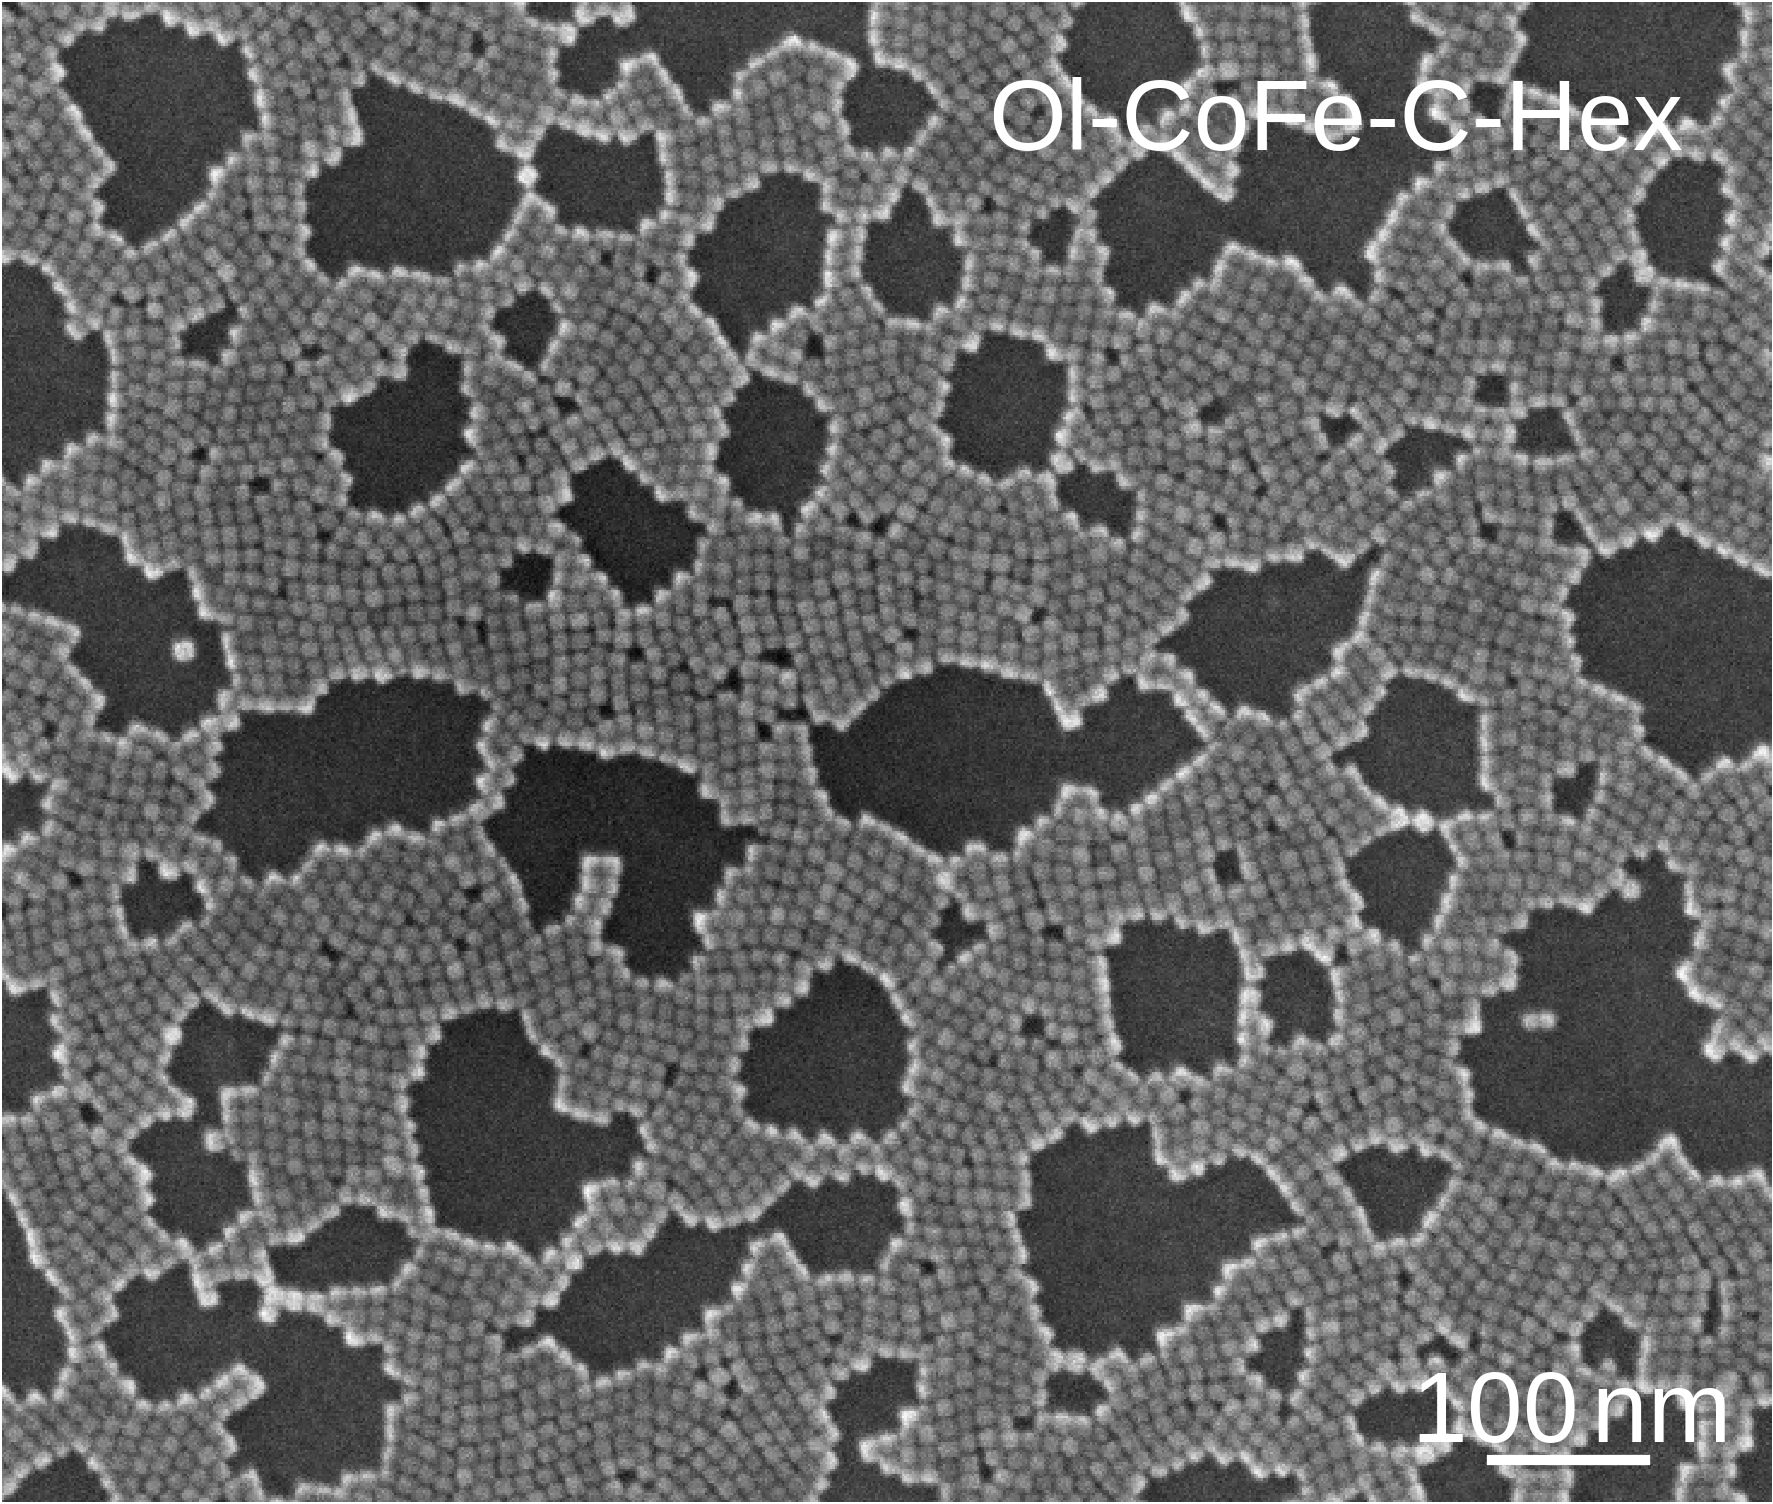
\includegraphics{monolayers_SEM_Ol-CoFe-C-Hex}
    \caption{\label{fig:monolayers:preparation:solventVariation:semNoCoSolvent}Scanning electron microscopy of Ol-CoFe-C nanoparticles after drop casting using only hexane and no co-solvent.}
  \end{figure}
  The solvent and co-solvent of the dispersion for the drop casting experiment determine the mobility of the nanoparticles and the time scales for the drop casting experiment.
  When oleic acid ligated nanocubes are drop casted as-prepared at low concentration from an organic dispersion such as n-hexane without any additional addends or setups, no long-range order is observed and the overall sample quality is inhomogeneous as seen in \reffig{fig:monolayers:preparation:solventVariation:semNoCoSolvent}.
  Early studies on drop casting of dodecanethiol-ligated gold nanospheres by Bigioni \etal \, show that a combination of toluene, a quickly evaporating solvent, as primary dispersion medium and a small fraction of dodecanethiol, a solvent with high-boiling point, as co-solvent results in long-range ordered nanostructure with spheres aligned on an hexagonal lattice \cite{Bigioni_2006_Kinet}.

  \subsubsection{Variation of Alkanes / Alkenes as Solvent / Co-Solvent}
    In this work, this idea has been transferred to oleic acid-ligated ferrite nanoparticles to prepare highly ordered monolayers.
    The influence of the choice of primary/co-solvent mixture is studied by performing drop casting experiments using the previously discussed nanocubes Ol-CoFe-C with varied alkane/alkene combinations.
    As primary solvent the alkane: \textit{n}-pentane, \textit{n}-hexane and \textit{n}-heptane are chosen for the rapidly evaporating component and for the high-boiling point addend the alkenes: 1-octadecene, 1-hexadecene, and 1-tetradecene were studied.
    For the experiment the nanoparticle concentration of the dispersions is set to $c_m \eq 0.13 \unit{mg/mL}$ and the co-solvent concentration to $c_V^\textsf{co} \eq 2\unit{Vol-\%}$.
    Scanning electron microscopy is performed (\refapp{app:additionalExperimentalTechniques:sem}) for a first evaluation of the samples and to study the local order.

    \begin{figure}[tb]
      \centering
      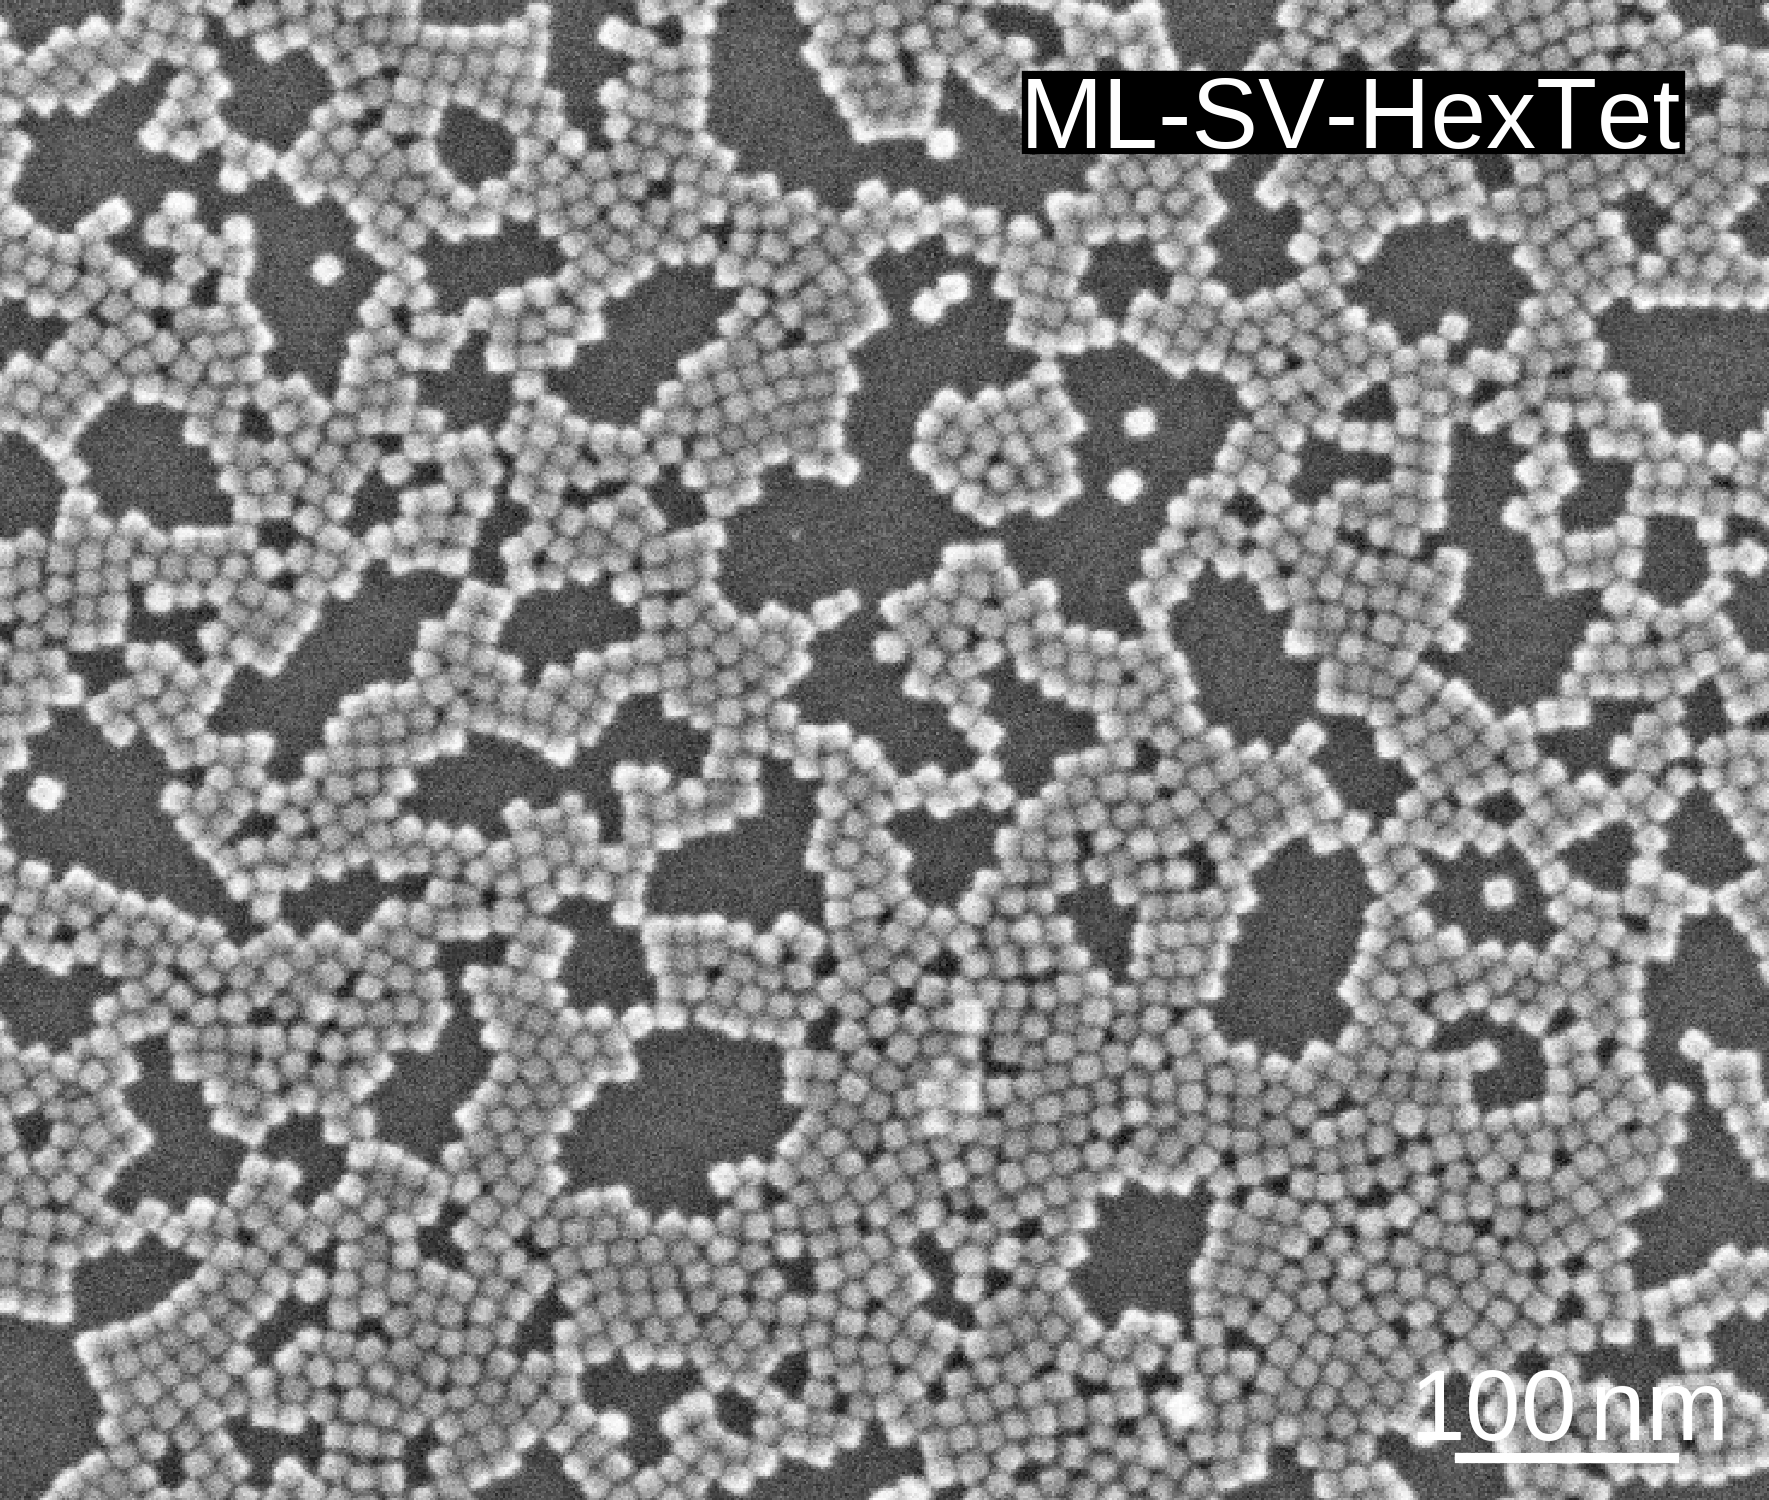
\includegraphics{monolayers_SEM_ML-SV-HexTet}
      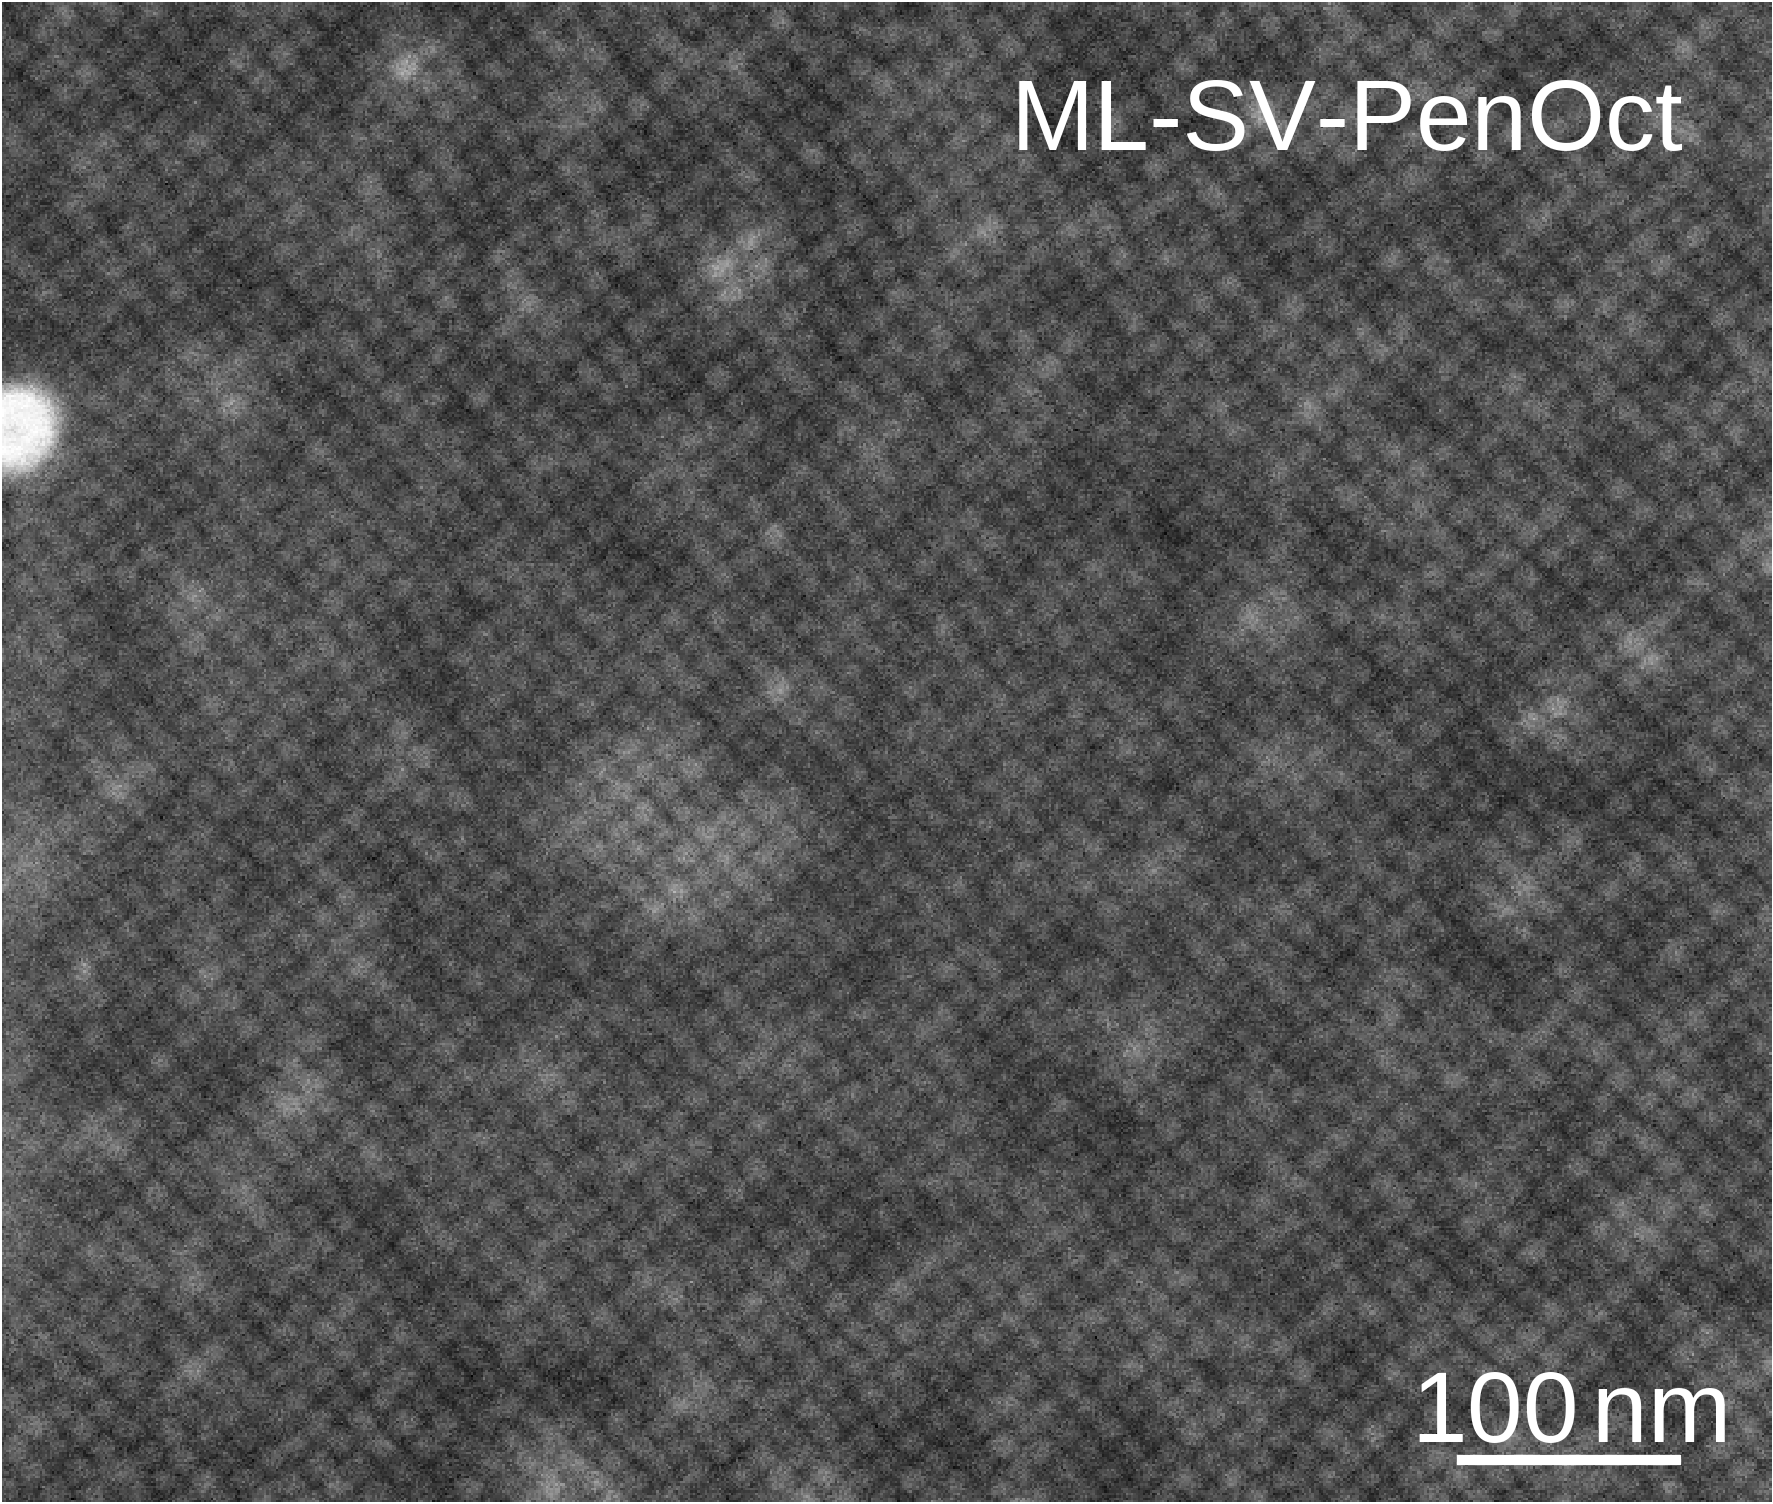
\includegraphics{monolayers_SEM_ML-SV-PenOct}
      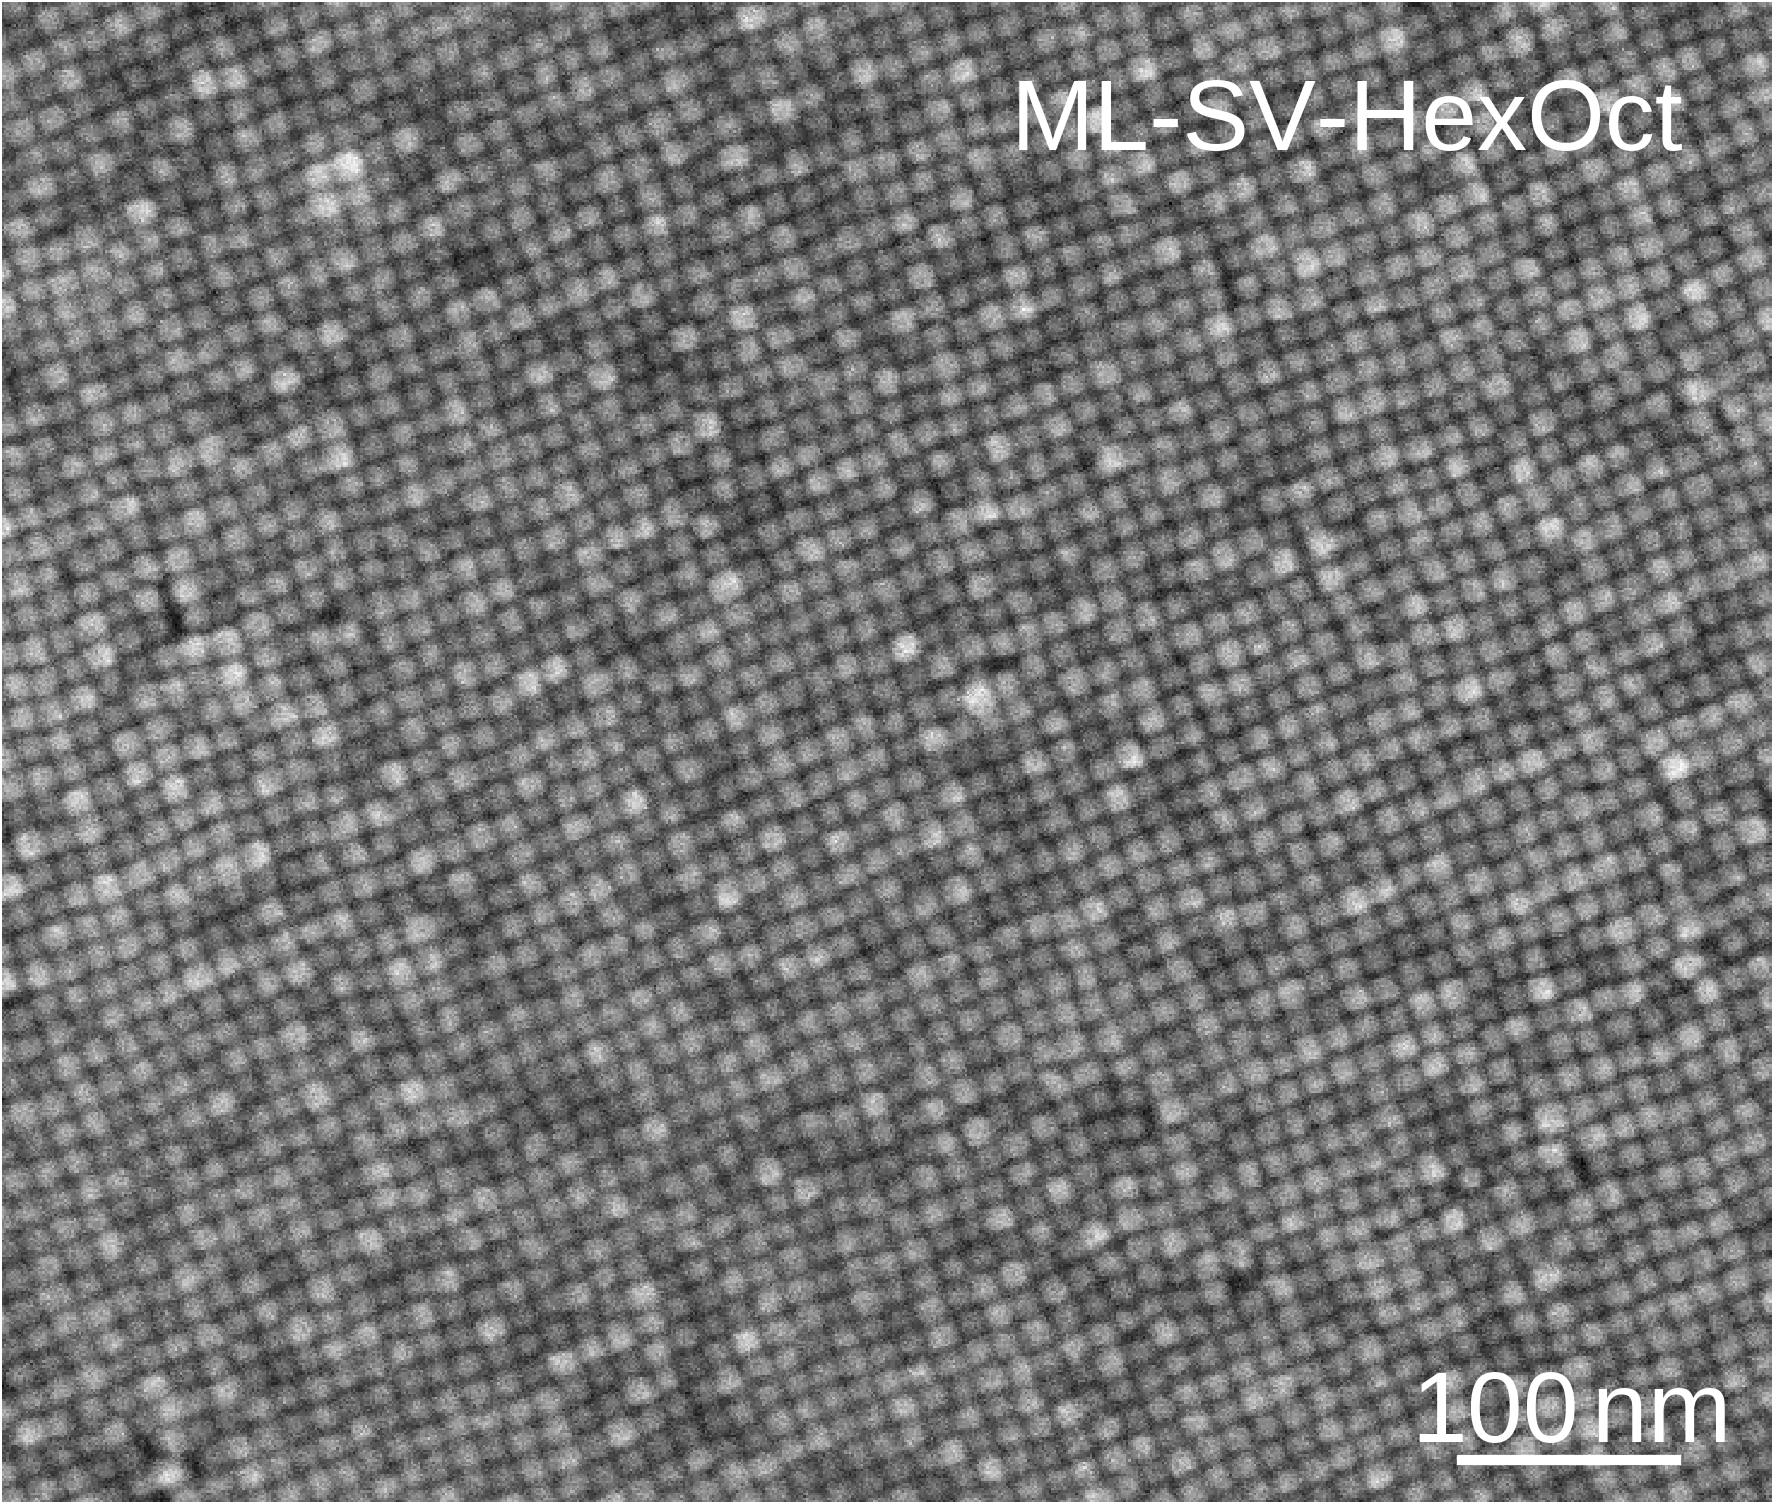
\includegraphics{monolayers_SEM_ML-SV-HexOct}
      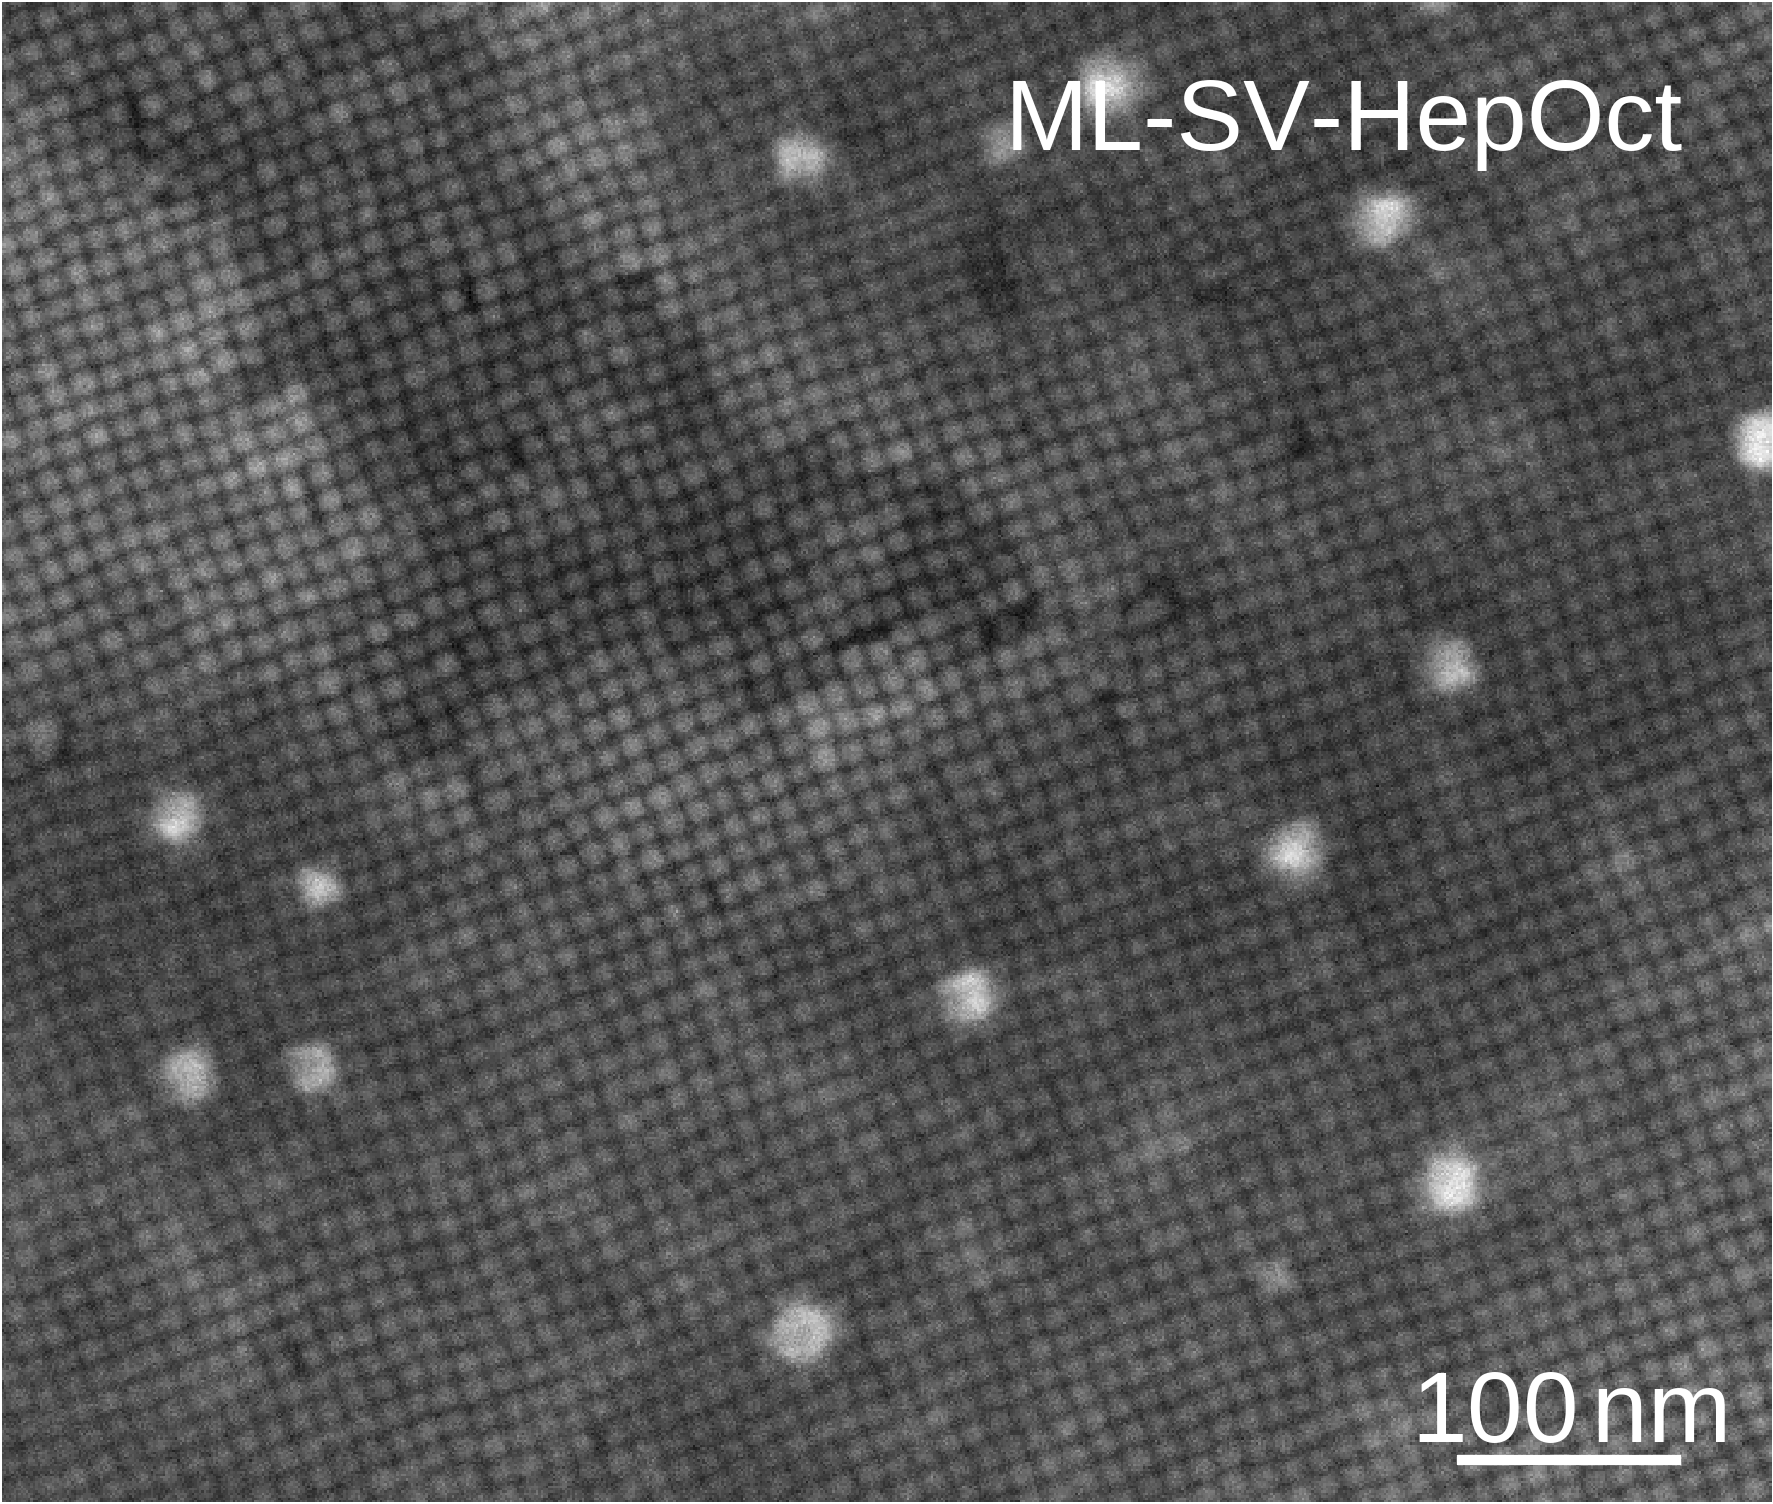
\includegraphics{monolayers_SEM_ML-SV-HepOct}
      \caption{\label{fig:monolayers:preparation:solventVariation:sem}Scanning electron microscopy of Ol-CoFe-C nanoparticles after drop casting using hexane/tetradecene (upper left),  pentane/octadecene (upper right), hexane/octadecene (lower left) and heptane/octadecene (lower right) as solvents.}
    \end{figure}

    \reffig{fig:monolayers:preparation:solventVariation:sem} shows four exemplary combinations: One sample to show a combination of an alkene with a relatively low boiling point, 1-tetradecene, together with \textit{n}-hexane (ML-SV-HexTet), and three samples to show combinations of 1-octadecene with the varied alkanes \textit{n}-pentane (ML-SV-PenOct), \textit{n}-hexane (ML-SV-HexOct) and \textit{n}-heptane (ML-SV-HepOct).
    A result that is imminently visible from SEM is that an alkene with a relatively low boiling point leads to no order formation, whereas  combinations with 1-octadecene show for all alkanes local square order formation.
    For the variation of the alkane component, the local evaluation of SEM images shows only minor qualitative differences.
    Thus to quantify the in-plane order, the selected samples are measured using grazing incidence small-angle X-ray scattering at GALAXI (\refapp{ch:appendix:lss:galaxi}).
    The resulting detector images are shown in \reffig{fig:monolayers:preparation:solventVariation:gisaxs}.
    As already visible in scanning electron microscopy, ML-SV-HexTet shows no significant structure factor along the Yoneda line, but mainly scattering coming from the form factor of the individual nanoparticles.
    For the other three shown samples, higher order alkanes show the emergence of structure peaks, where the relative intensity of the first order peak in the Yoneda line increases with the order of the alkane which is visible in the lower panels of \reffig{fig:monolayers:preparation:solventVariation:gisaxs}.

    \begin{figure}[tb]
      \centering
      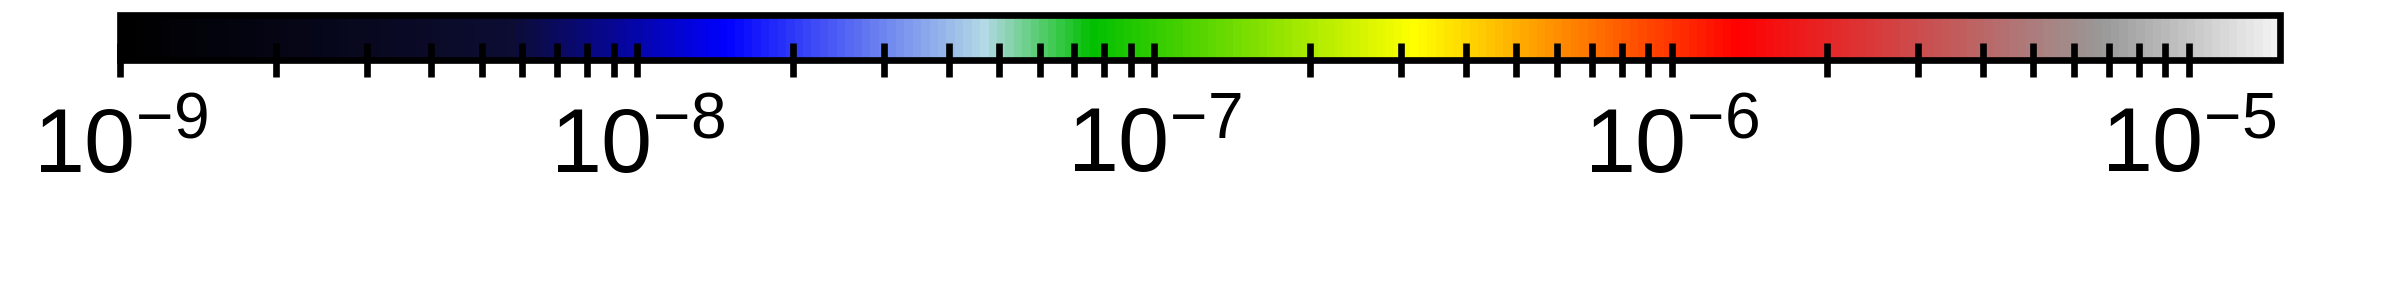
\includegraphics{monolayers_GISAXS_SVcbar}
      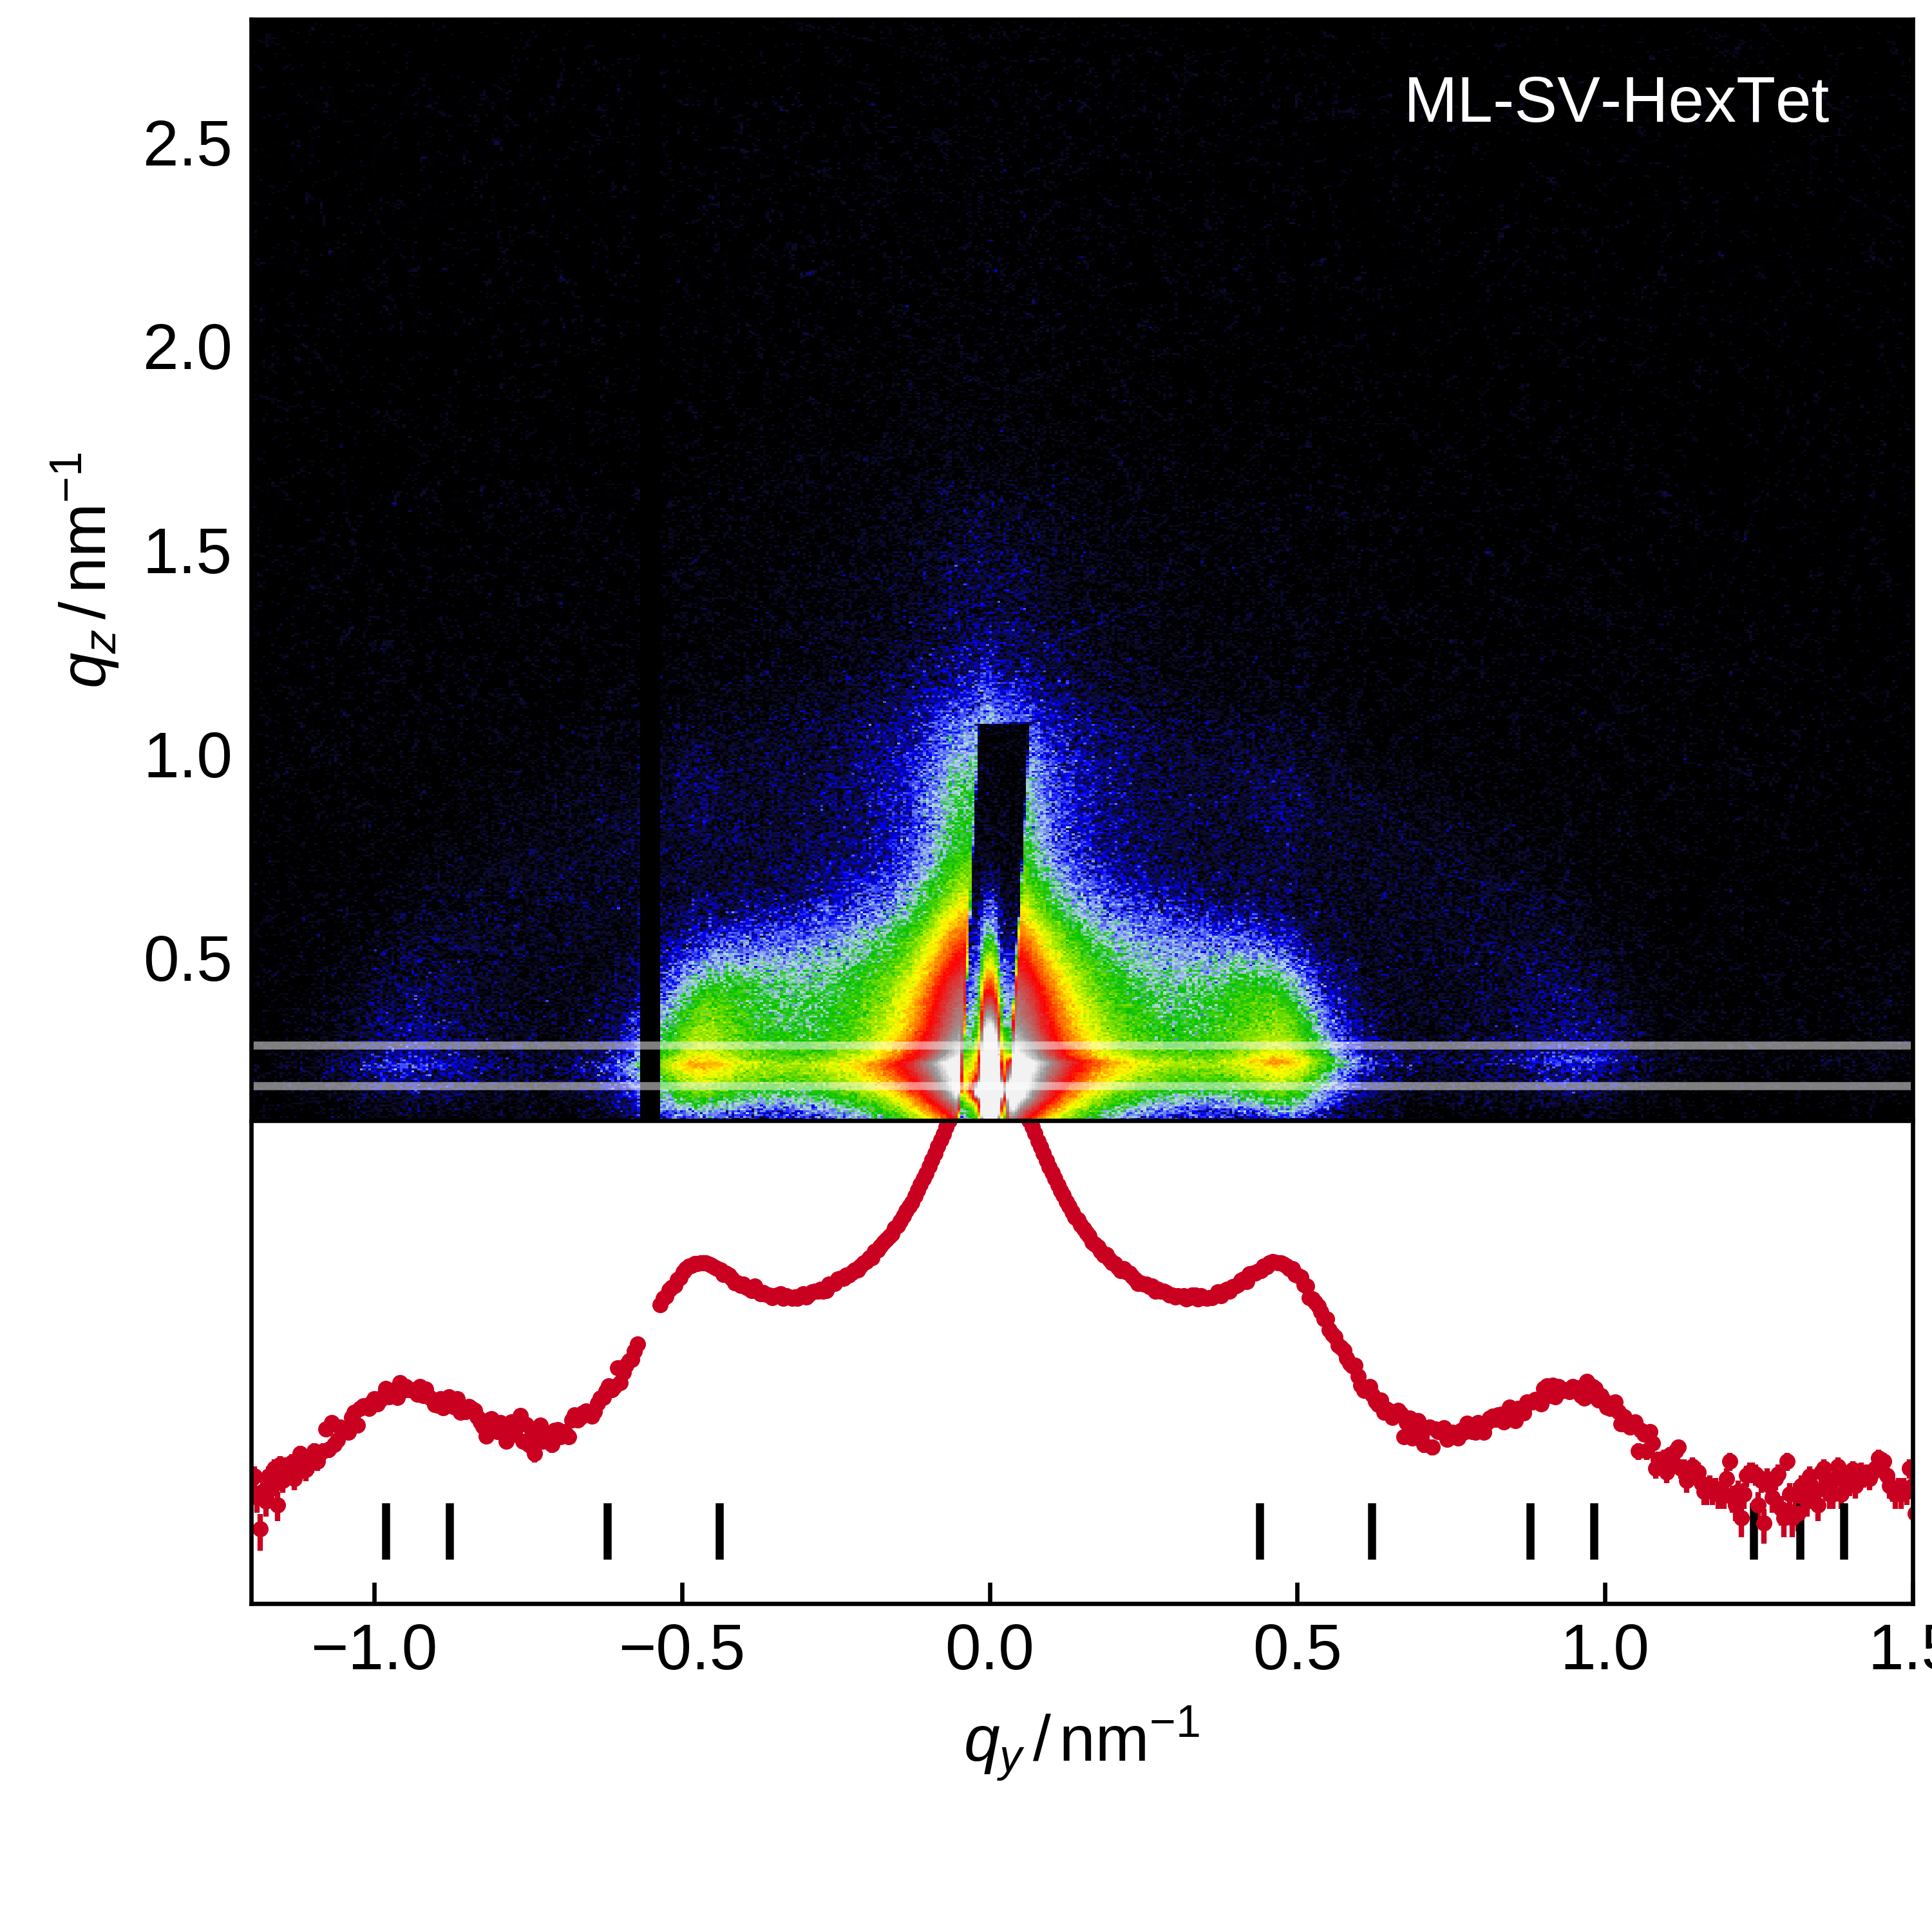
\includegraphics{monolayers_GISAXS_ML-SV-HexTet}
      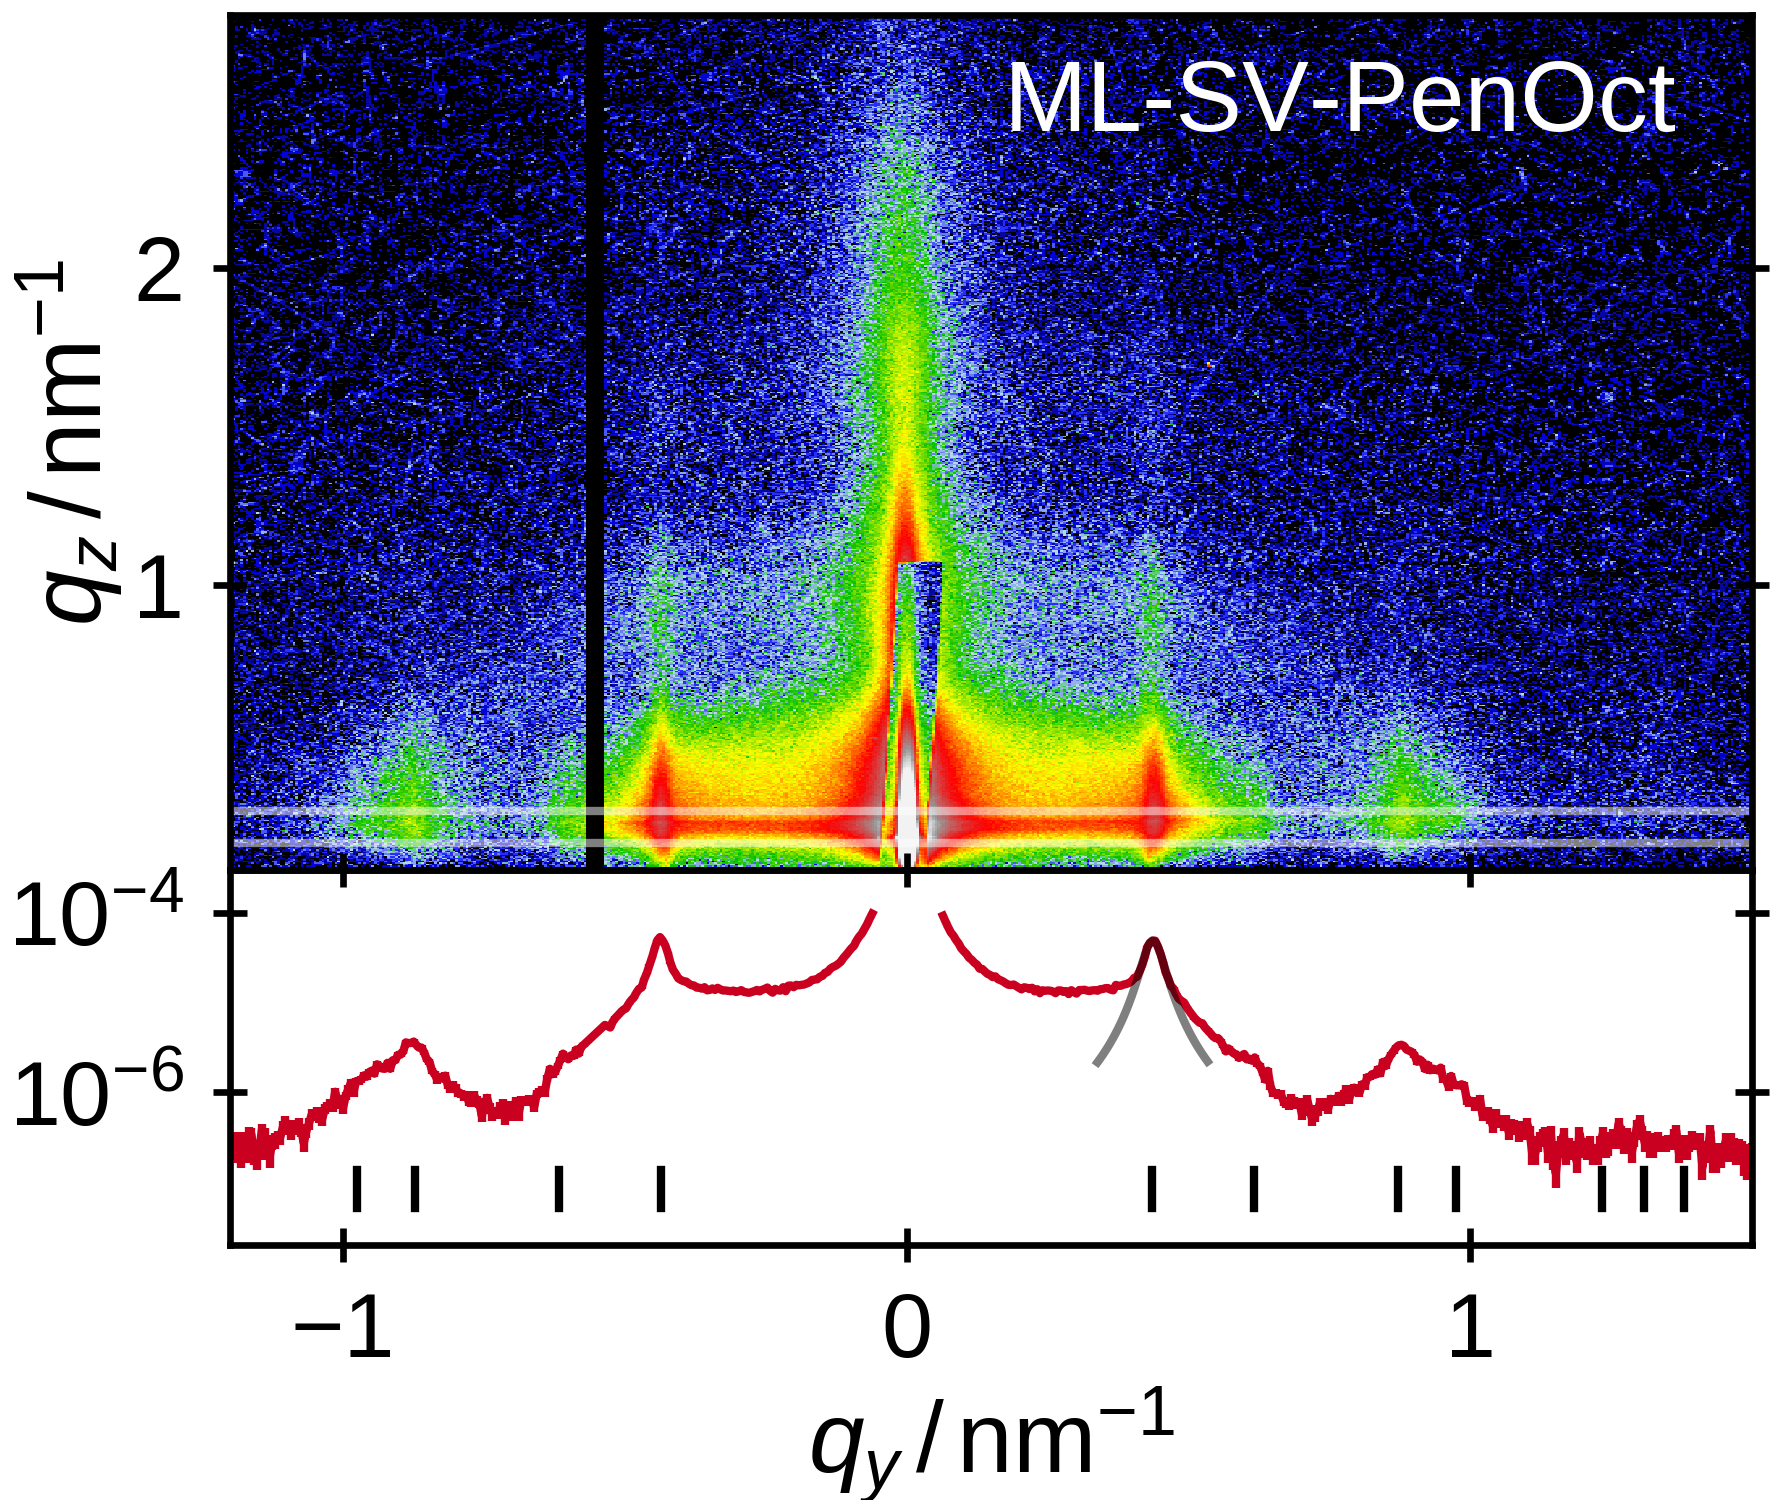
\includegraphics{monolayers_GISAXS_ML-SV-PenOct}
      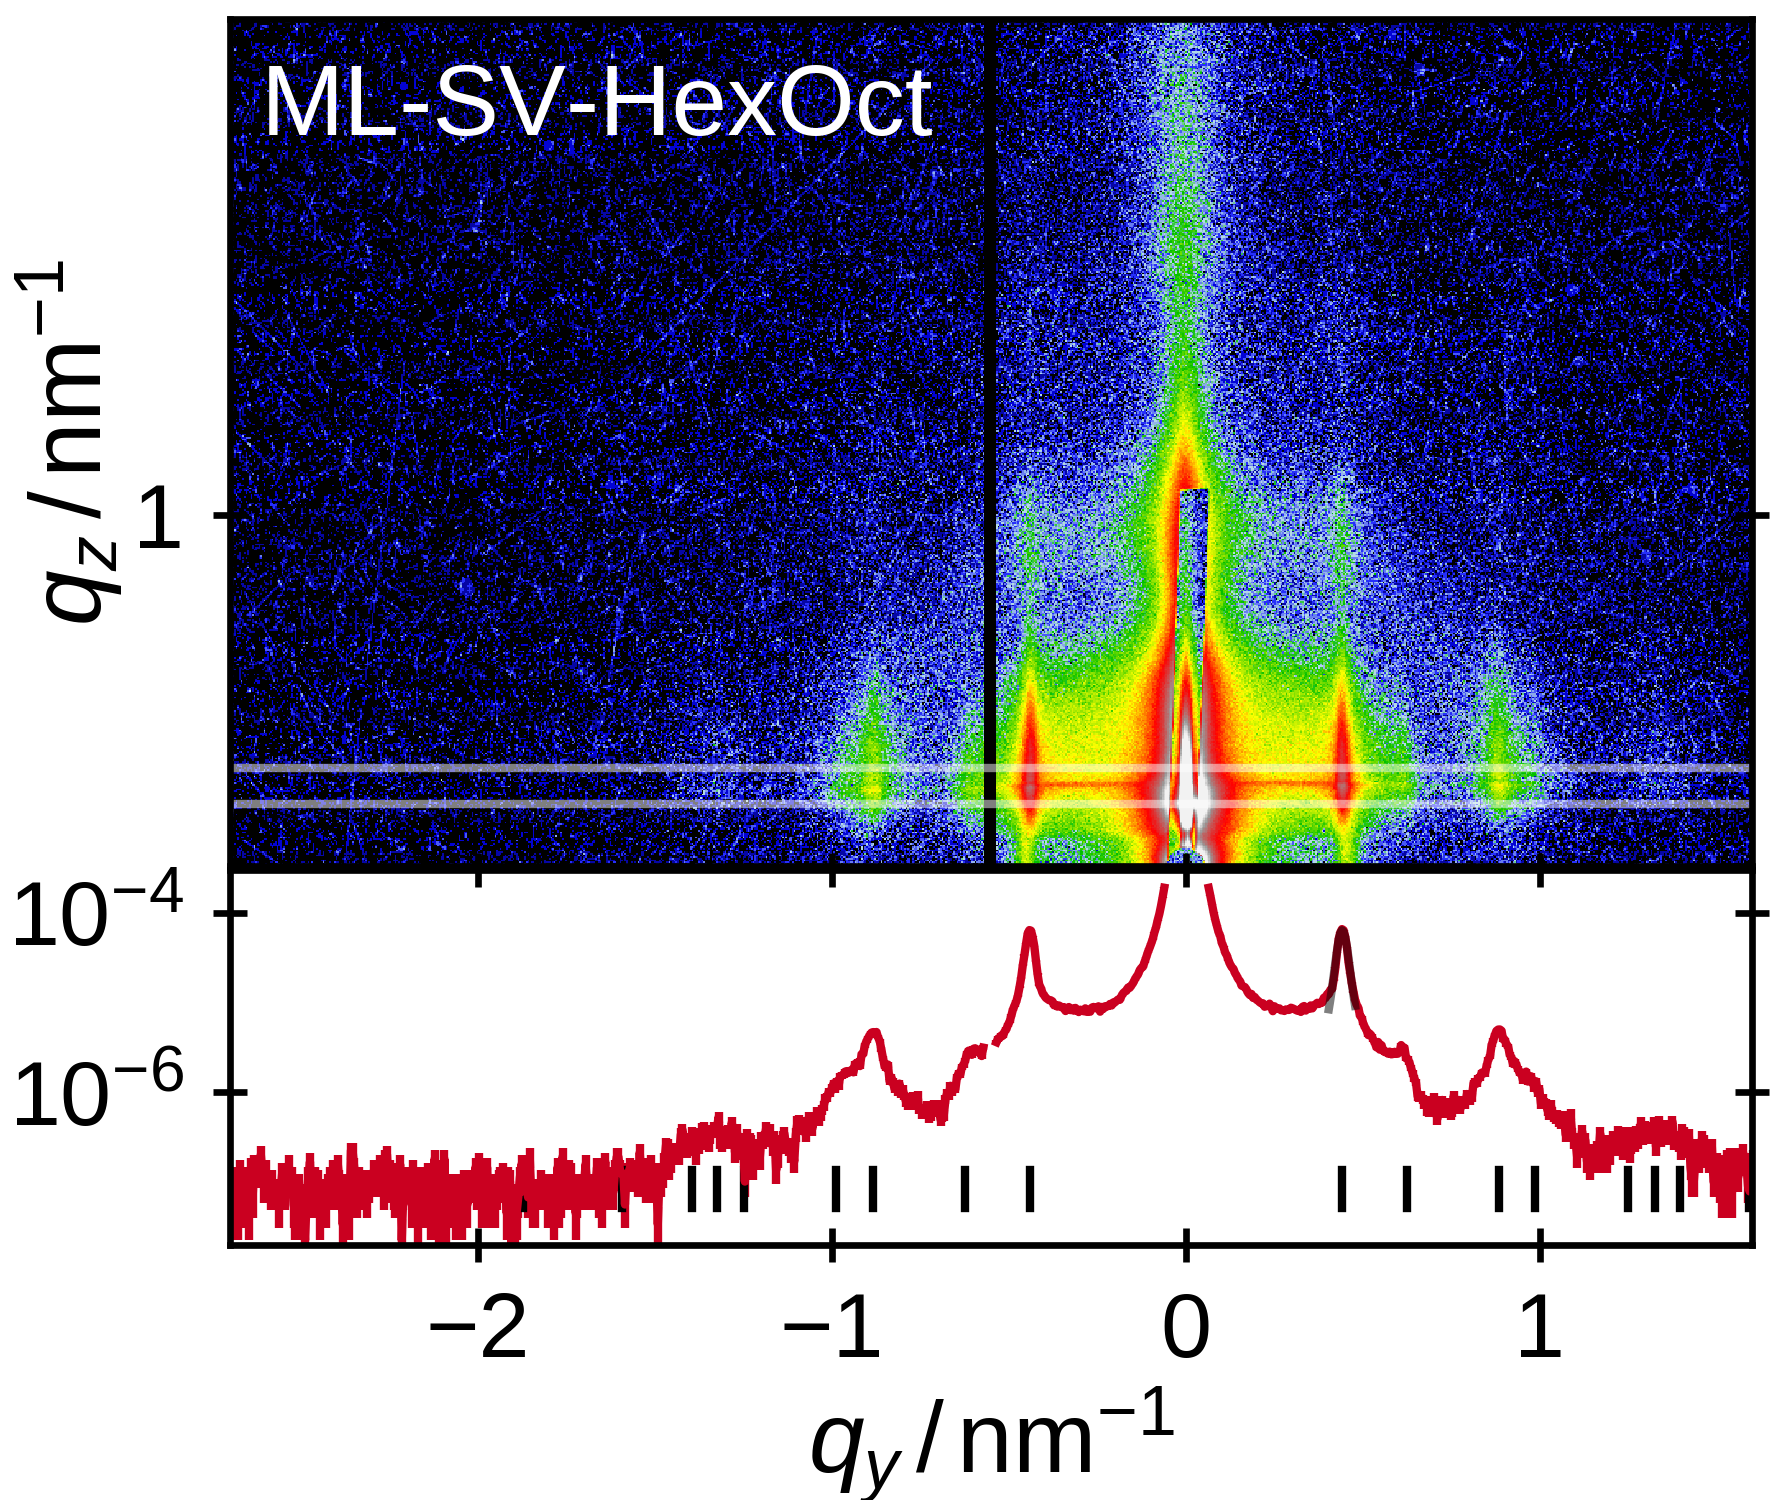
\includegraphics{monolayers_GISAXS_ML-SV-HexOct}
      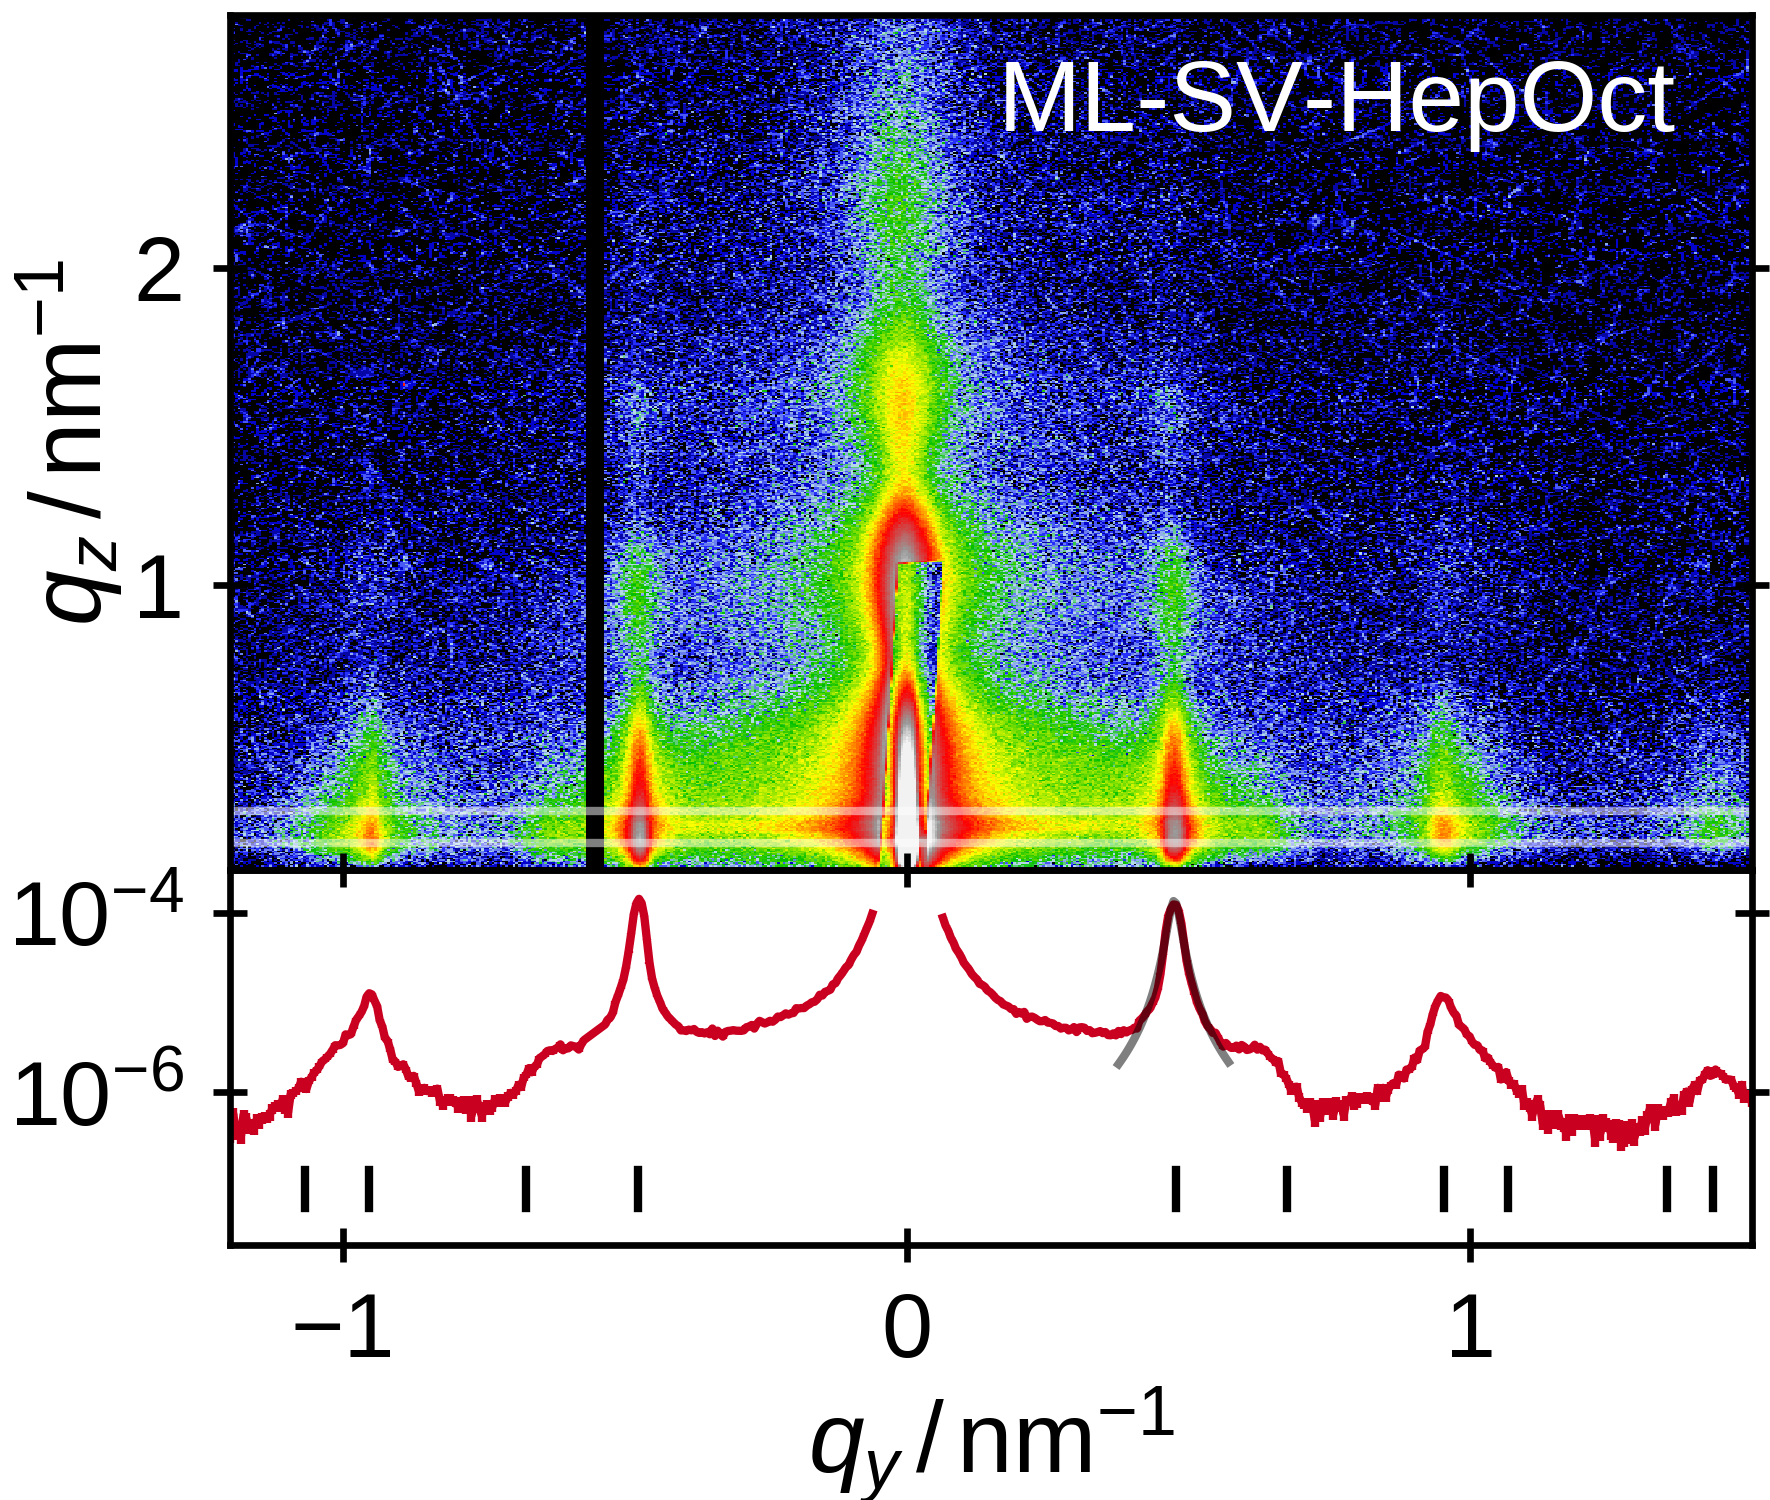
\includegraphics{monolayers_GISAXS_ML-SV-HepOct}
      \caption{\label{fig:monolayers:preparation:solventVariation:gisaxs}GISAXS detector images measured under an incident angle of $\alpha_i \eq 0.11 \unit{^\circ}$ to study the average lateral structure of the samples shown in \reffig{fig:monolayers:preparation:solventVariation:sem}. Below the detector images, the respective scattered intensity in the strip around the Yoneda line is shown. For the ordered samples, the first order peak is fitted to a Lorentzian function with the parameters tabulated in \reftab{tab:monolayers:solventProperties:GisaxsLatticeParams}.}
    \end{figure}

    The peak positions are compared to the expected relative positions for a square lattice, given by
    \begin{align}
      q_{hk} \eq \frac{2 \pi}{a} \sqrt{h^2 + k^2},
    \end{align}
    where $h$, $k$ are integers and $a$ the lattice constant of the square arrangement, which is estimated from the (10) peak position.
    For ML-SV-HexOct the position of all peaks fits to this pattern, whereas for ML-SV-PenOct and ML-SV-HepOct the (11) peak position is less visible.
    This effect can be attributed to the unlucky coincidence that the (11) peak position is within the formfactor minima in these cases.
    \FloatBarrier

    \begin{table}[tb]
      \centering
      \caption{\label{tab:monolayers:solventProperties:GisaxsLatticeParams}Position and width of the first order peak observed in the GISAXS detector images in \reffig{fig:monolayers:preparation:solventVariation:gisaxs}.}
      \begin{tabular}{ c || l | l || l | l }
        Sample  & $q_{10}$ / $\unit{nm^{-1}}$ & $\Delta q_{10}$ / $nm^{-1}$ & $a$ / nm & $d_{coh.}$ / nm \\
        \hline
        ML-SV-PenOct
          & $0.4367(3)$
          & $0.042(1)$
          & $14.39(1)$
          & $1061(35)$\\
        ML-SV-HexOct
          & $0.4342(1)$
          & $0.030(1)$
          & $14.22(1)$
          & $1721(86)$\\
        ML-SV-HepOct
          & $0.4747(6)$
          & $0.024(2)$
          & $13.24(2)$
          & $2662(477)$\\
        \hline
      \end{tabular}
    \end{table}

    Within the theory of paracrystals, GISAXS provides a direct measure of the lattice constant and the coherence length of the square lattice via the position and the inverse width of the structure factor peaks \cite{Renaud_2009_Probi}.
    For Gaussian disorder of the nearest neighbor position, the peak broadening is described by a Lorentzian function as shown in \refapp{ch:appendix:calculations:paracrystal}
    \begin{align}
      I(q_y) \eq \frac{A} {1 + \biggl(2\frac{q_y - q_{10}}{\Delta q_{10}}\biggr)^2},
    \end{align}
    which has as parameters the intensity $A$ of the (10) peak with position $q_{10}$ and FWHM $\Delta q_{10}$.
    And the lattice constant and coherence length is given by
    \begin{align}
      a &\eq \frac{2 \pi}{q_{10}}, \\
      d_{coh.} &\eq \frac{4 \pi^2}{\sqrt{ \Delta q_{10}^2 - \Delta q_{D.B.}^2 }},
    \end{align}
    where the FWHM of the peak is corrected for $\Delta q_{D.B.} \eq 0.0195(7) \unit{nm^{-1}}$, the FWHM of the direct beam, which is given in \reffig{fig:appendix:lss:galaxi:directBeam}.
    In \reftab{tab:monolayers:solventProperties:GisaxsLatticeParams}, the position and width of the first order peak for the three different samples prepared with 1-octadecene is listed.

    The table shows that for increasing order of alkane, the lattice constant reduces and the coherence length increases.
    Both can be explained by an improved packing of the square lattice and therefore this is in agreement with the qualitative observation that higher alkanes increase the sample quality.
    A further qualitative assessment of a combination from \textit{n}-octane/1-octadecene (not shown) shows that the long-range order decreases again significantly.
    As well as that the combination \textit{n}-heptane/1-hexadecene is of lower quality.
    Combinations using higher order alkenes are not feasible at ambient conditions, as the freezing point of the alkenes with longer C-chain than 1-octadecene is above room temperature and therefore they are solid.

    In summary, the best quality of samples from a series of alkane/alkene combinations is achieved for a combination of \textit{n}-heptane together with small addends of 1-octadecene.
    An approach to explain this specific combination can be given by the freezing point of 1-octadecene and the evaporative cooling properties of \textit{n}-heptane.
    1-octadecene freezes at a temperature of approx. $15 \unit{^\circ C}$, whereas evaporating \textit{n}-heptane and lower order alkanes can cool by over $\Delta T \eq 10 \unit{^\circ C}$ due to evaporative cooling \cite{Tuckermann_2002_Evapo}.
    Thus, it can be assumed that during evaporation of the quickly evaporating \textit{n}-heptane at room temperature ($T \eq 22 \unit{^\circ C}$ measured for the laboratory surfaces), the surface of the droplet is cooled near the freezing temperature of 1-octadecene, which increases the viscosity of the liquid at the surface.
    This generates the condition needed for monolayer formation as described in \cite{Bigioni_2006_Kinet}, where particles are pinned to the surface of the evaporating droplet at which they can find one another to form a single ordered layer.
    Increasing the order of the alkane reduces the evaporative cooling effect from the drop casting experiment, as to why there is no order observed for alkanes higher than \textit{n}-heptane.
    Decreasing the order of the alkane, increases the evaporative cooling effect, but also decreases the time the particles have to order themselves with great mobility.
    On the other hand, exchanging 1-octadecene for a lower order alkene reduces the freezing point, as to which no long-range order is observed.

    \begin{figure}[tb]
      \centering
      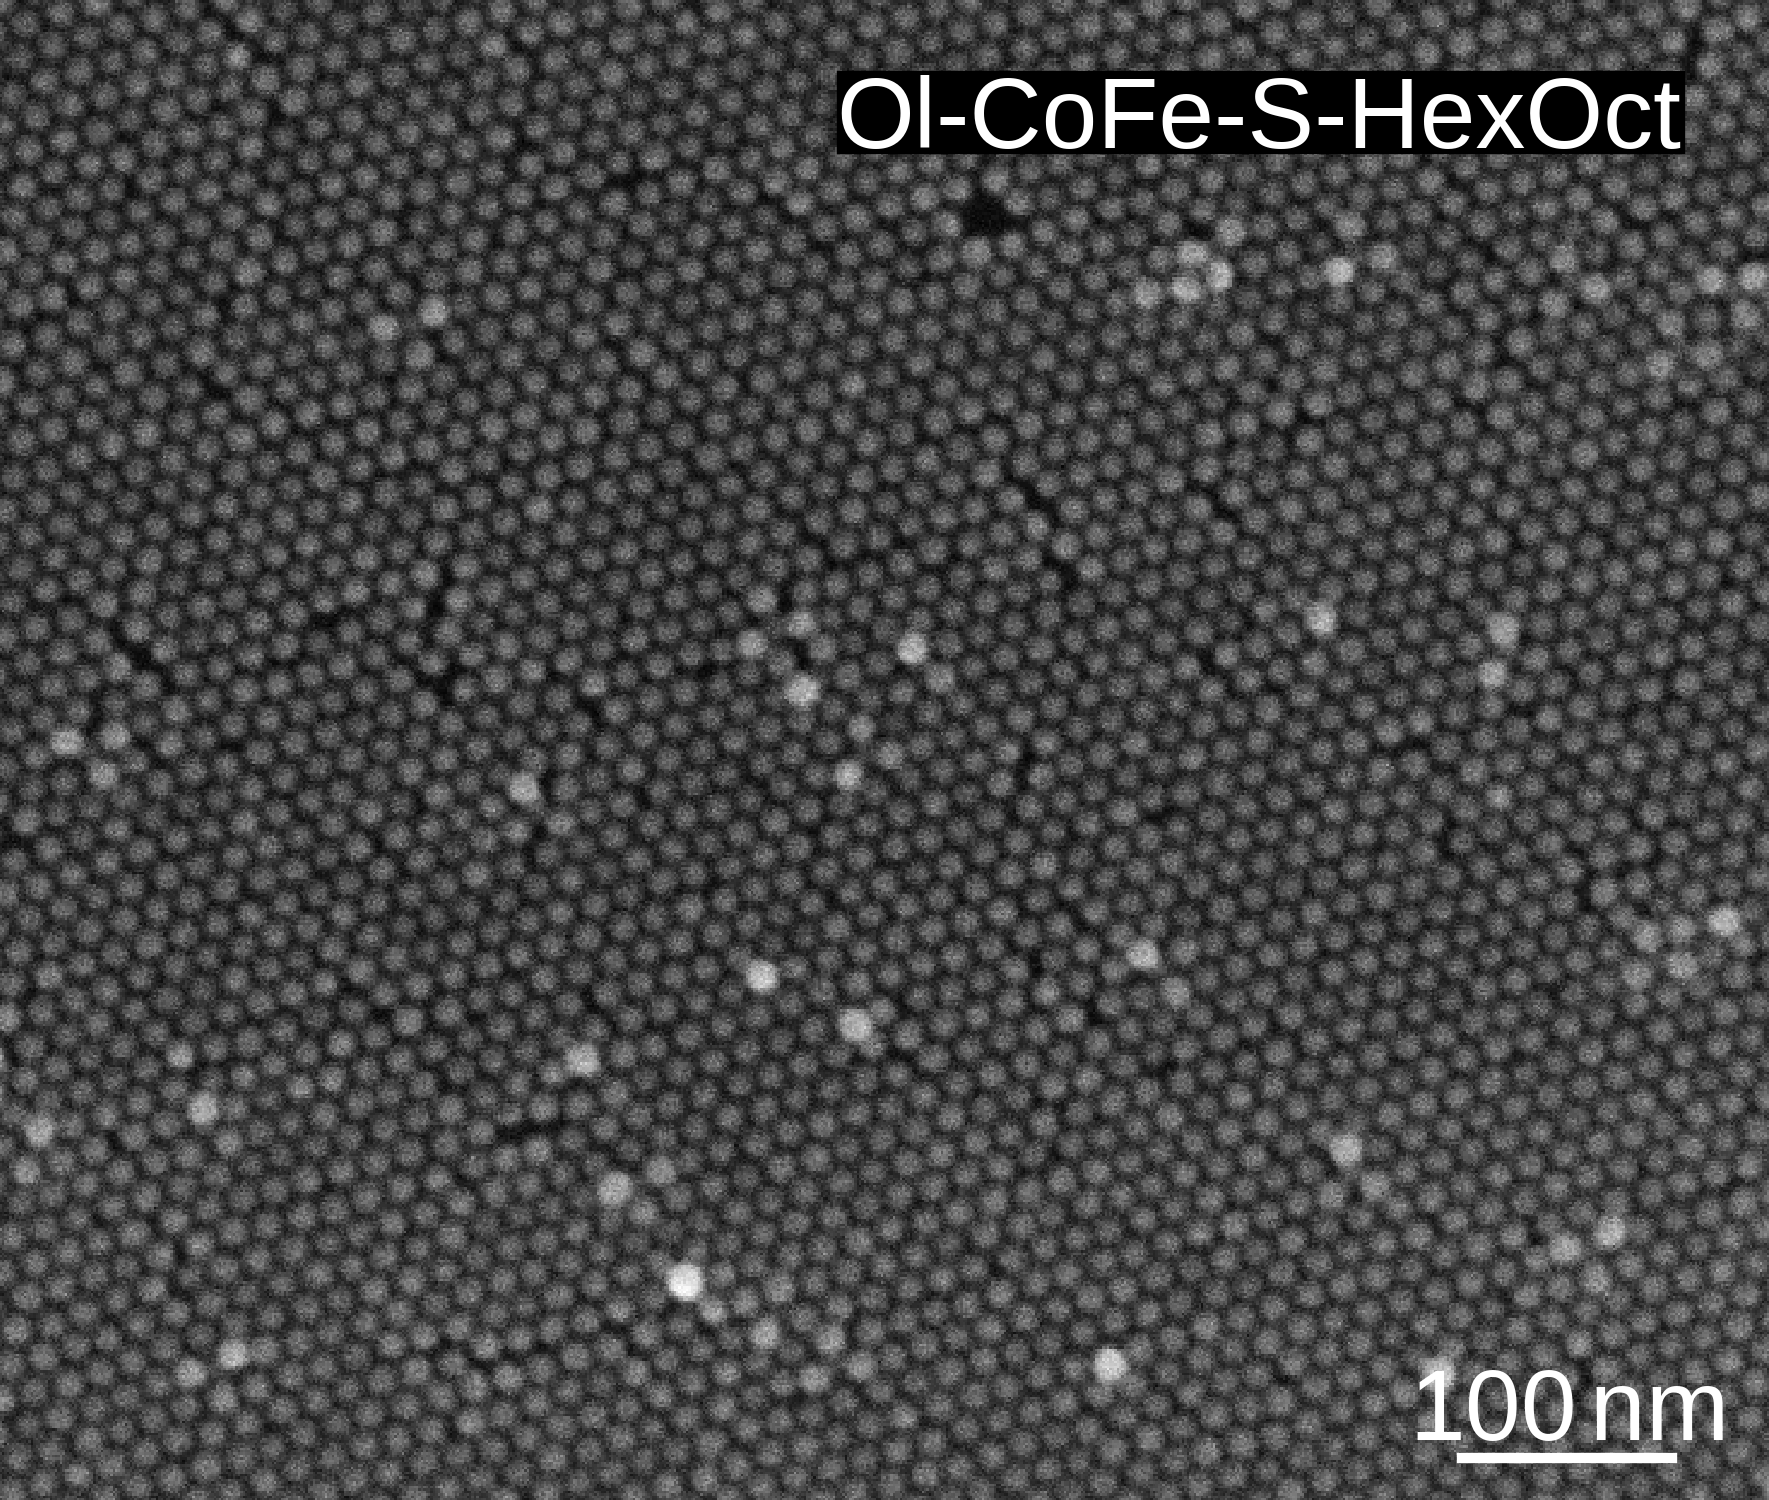
\includegraphics{monolayers_SEM_Ol-CoFe-S-HexOct}
      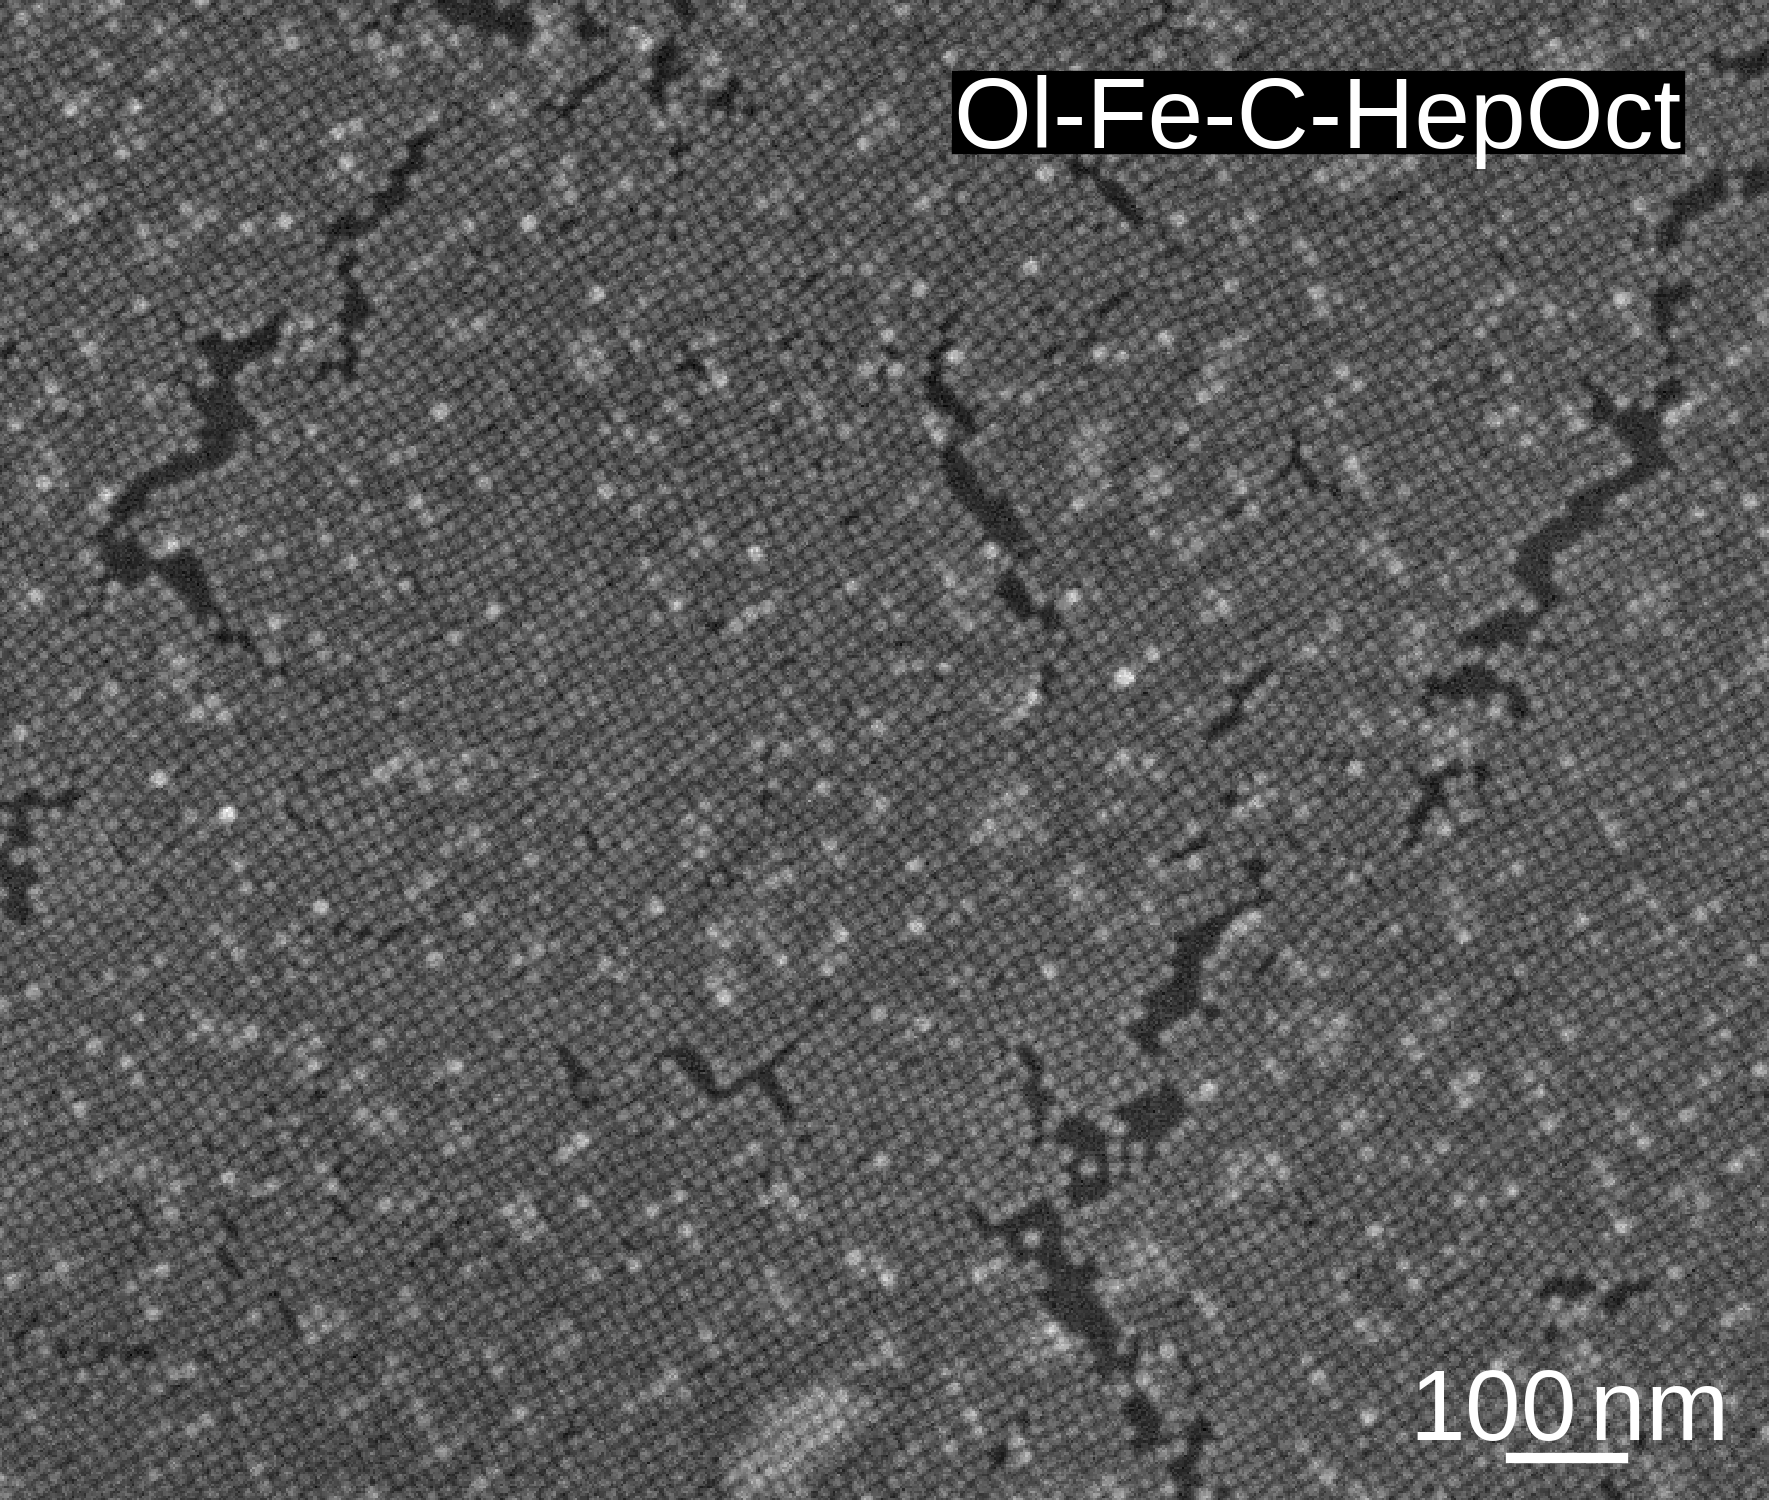
\includegraphics{monolayers_SEM_Ol-Fe-C-HepOct}
      \caption{\label{fig:monolayers:preparation:solventVariation:spheresIron}Scanning electron microscopy of other type of nanoparticles deposited as monolayers also using 1-octadecene as co-solvent. Shown is the structure of cobalt ferrite nanospheres (left) and iron oxide nanocubes (right).}
    \end{figure}

  \subsubsection{Oleic Acid Addend}
    These combinations were also transferred to various other oleic acid ligated nanoparticles during this work, such as cobalt ferrite nanospheres or iron oxide nanocubes as exemplary shown in \reffig{fig:monolayers:preparation:solventVariation:spheresIron}.
    From varied success rates during the transfer to other nanoparticles it became apparent that the oleic acid content within the dispersion is also a crucial part for the monolayer formation, especially for particles synthesized following the acetylacetonate route.

    \begin{figure}[tb]
      \centering
      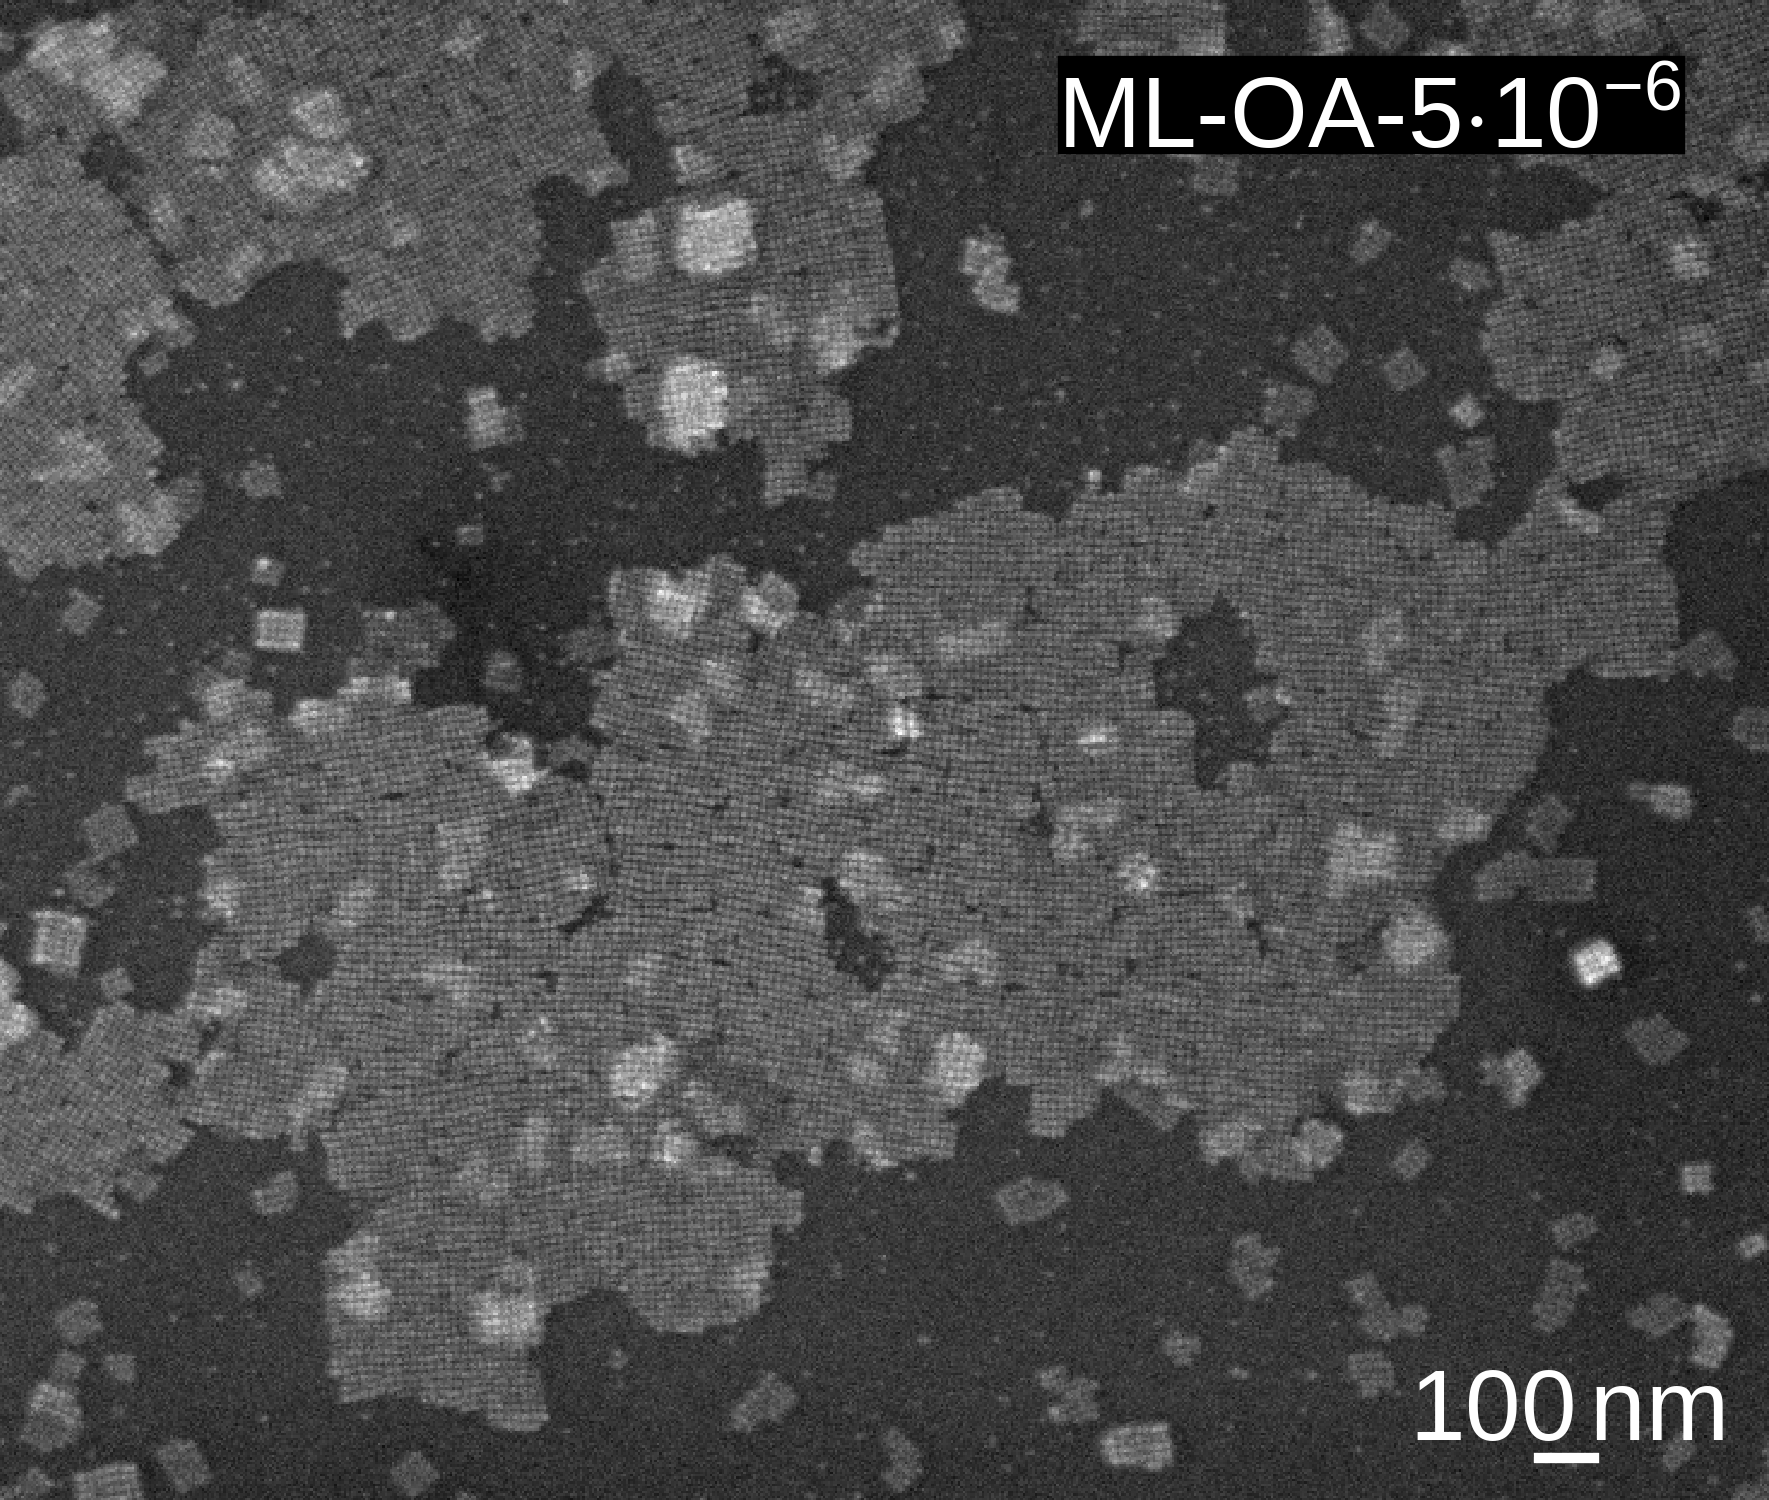
\includegraphics{monolayers_SEM_ML-OA-5e-6}
      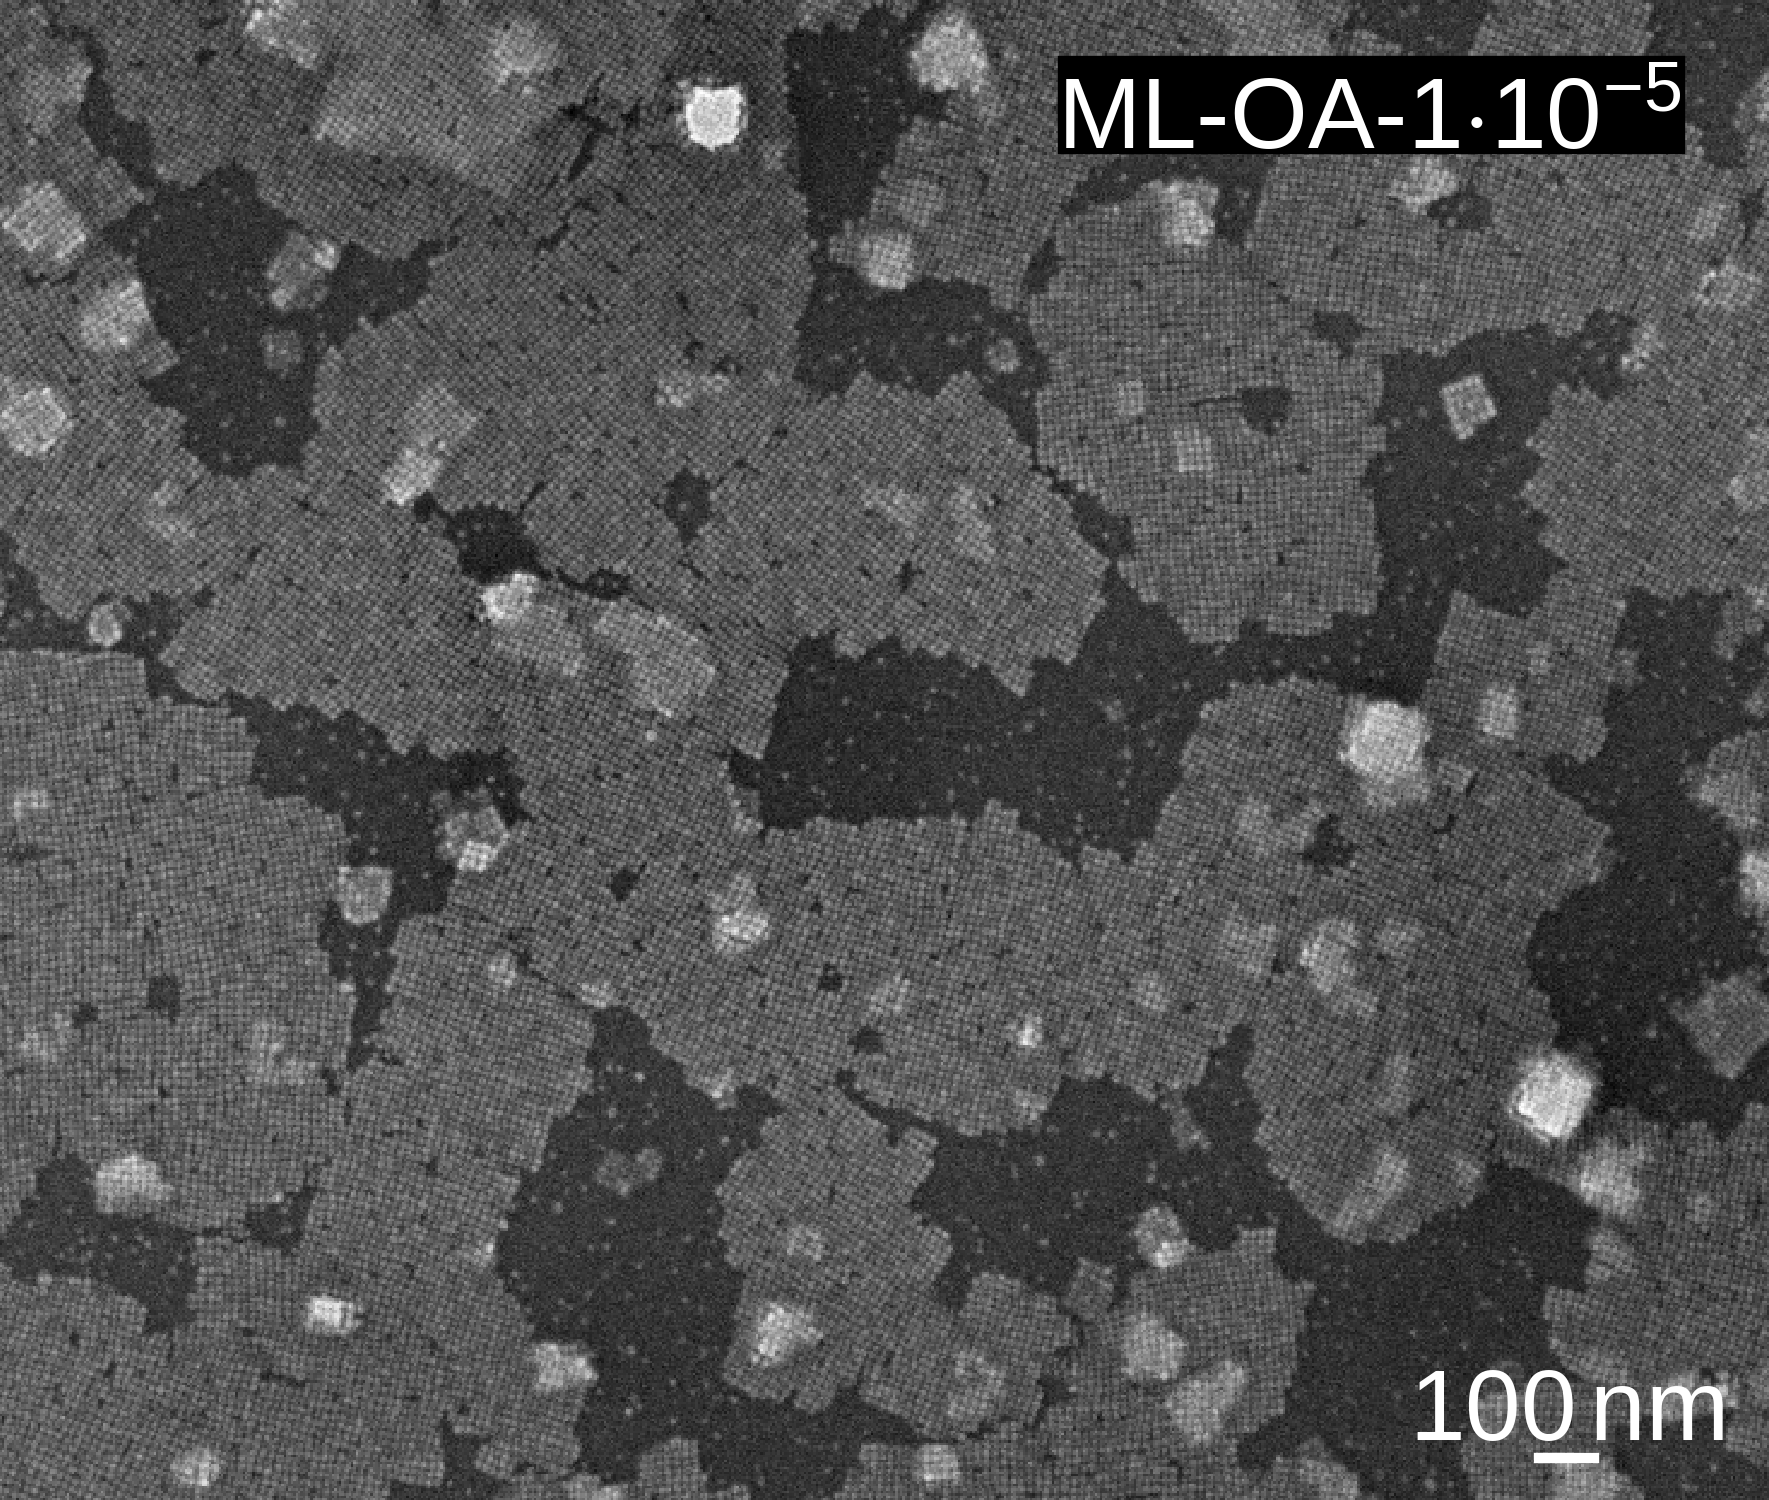
\includegraphics{monolayers_SEM_ML-OA-1e-5}
      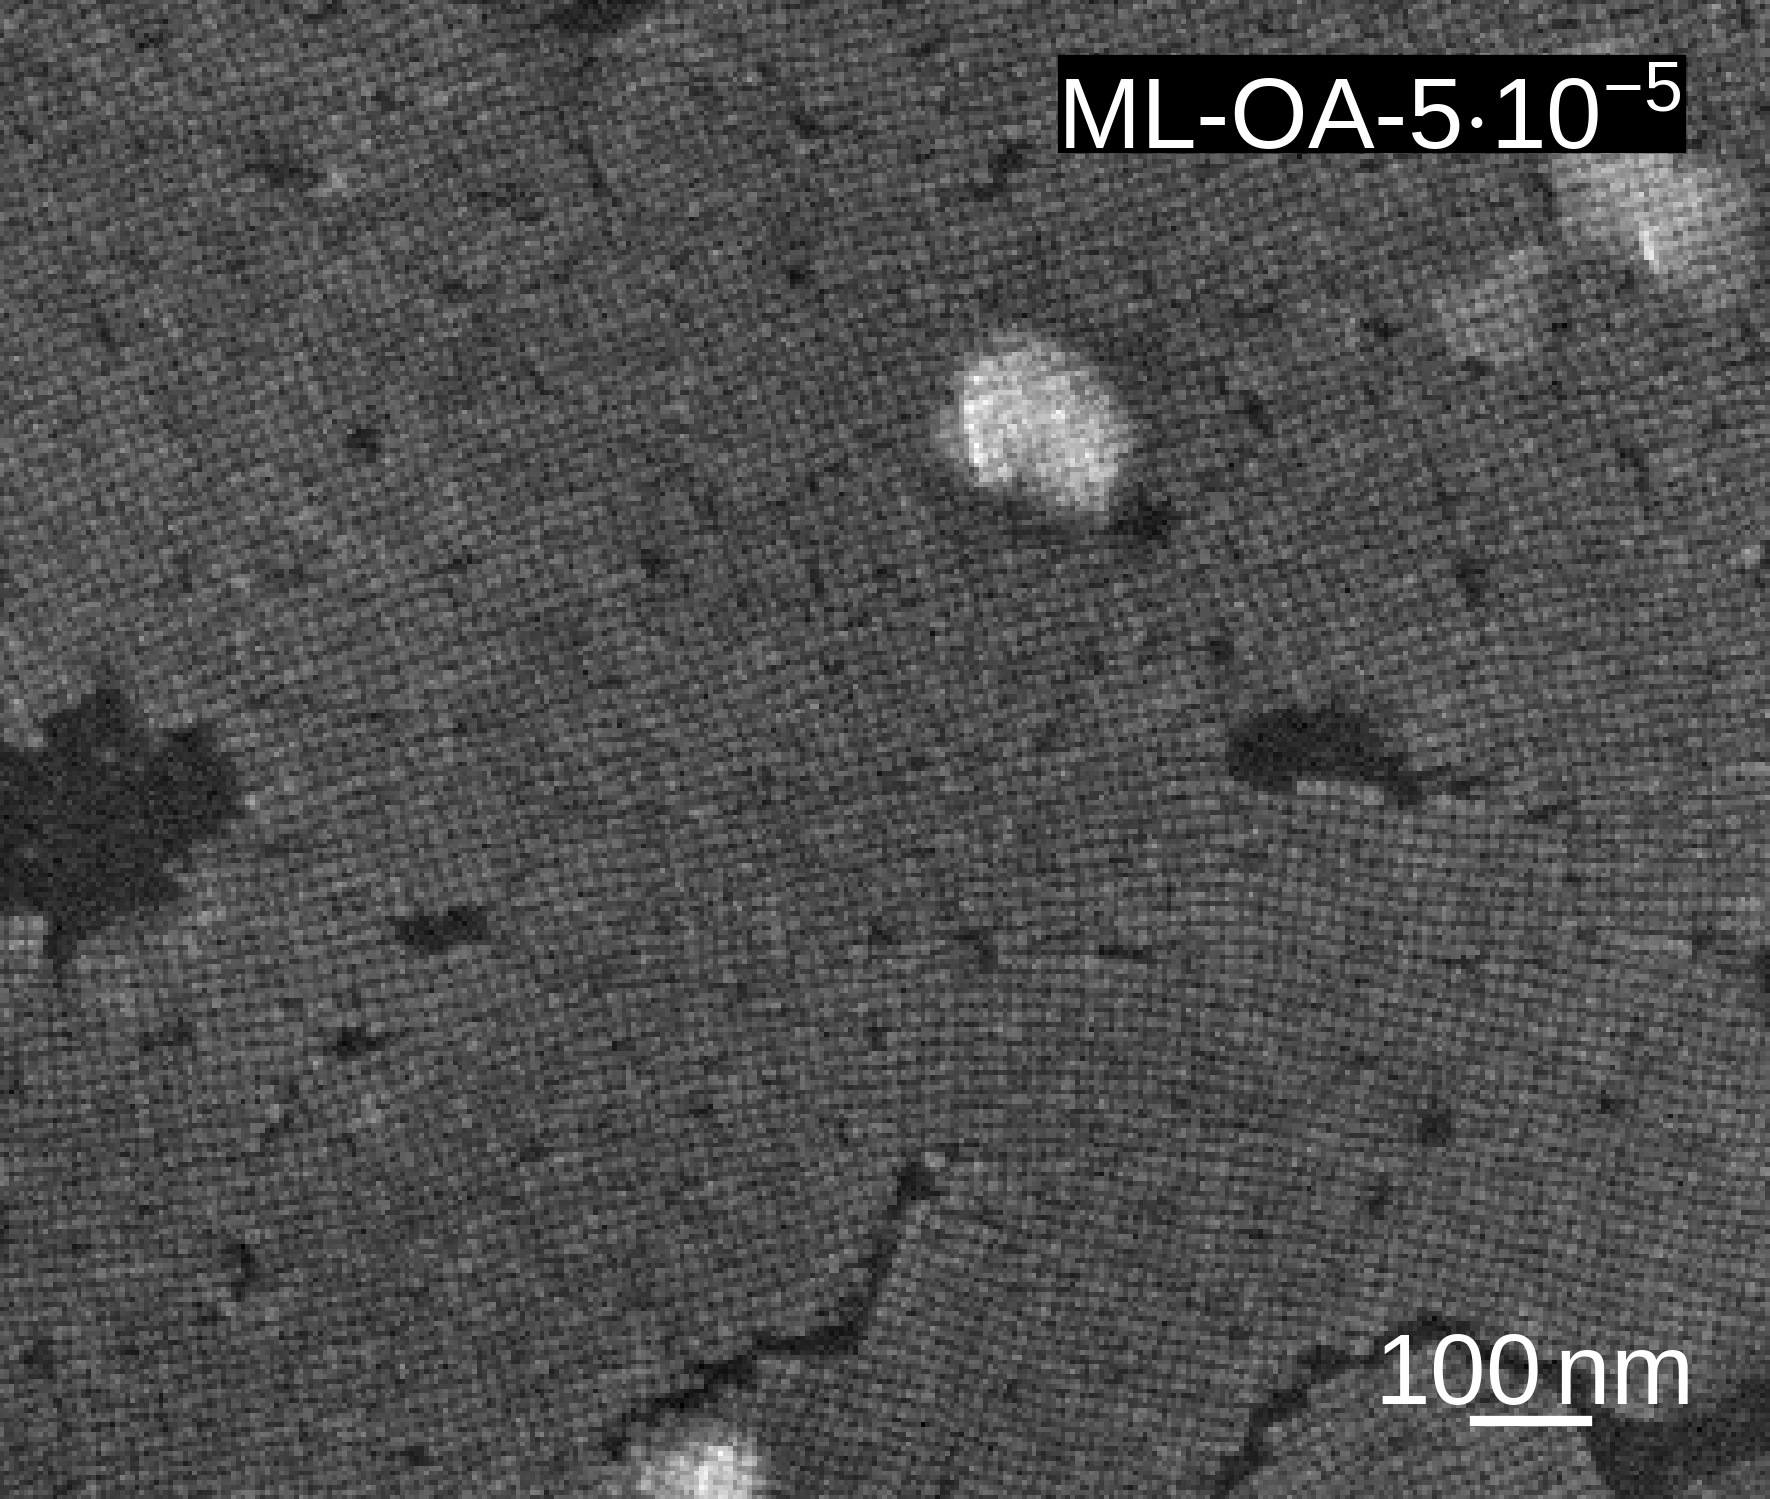
\includegraphics{monolayers_SEM_ML-OA-5e-5}
      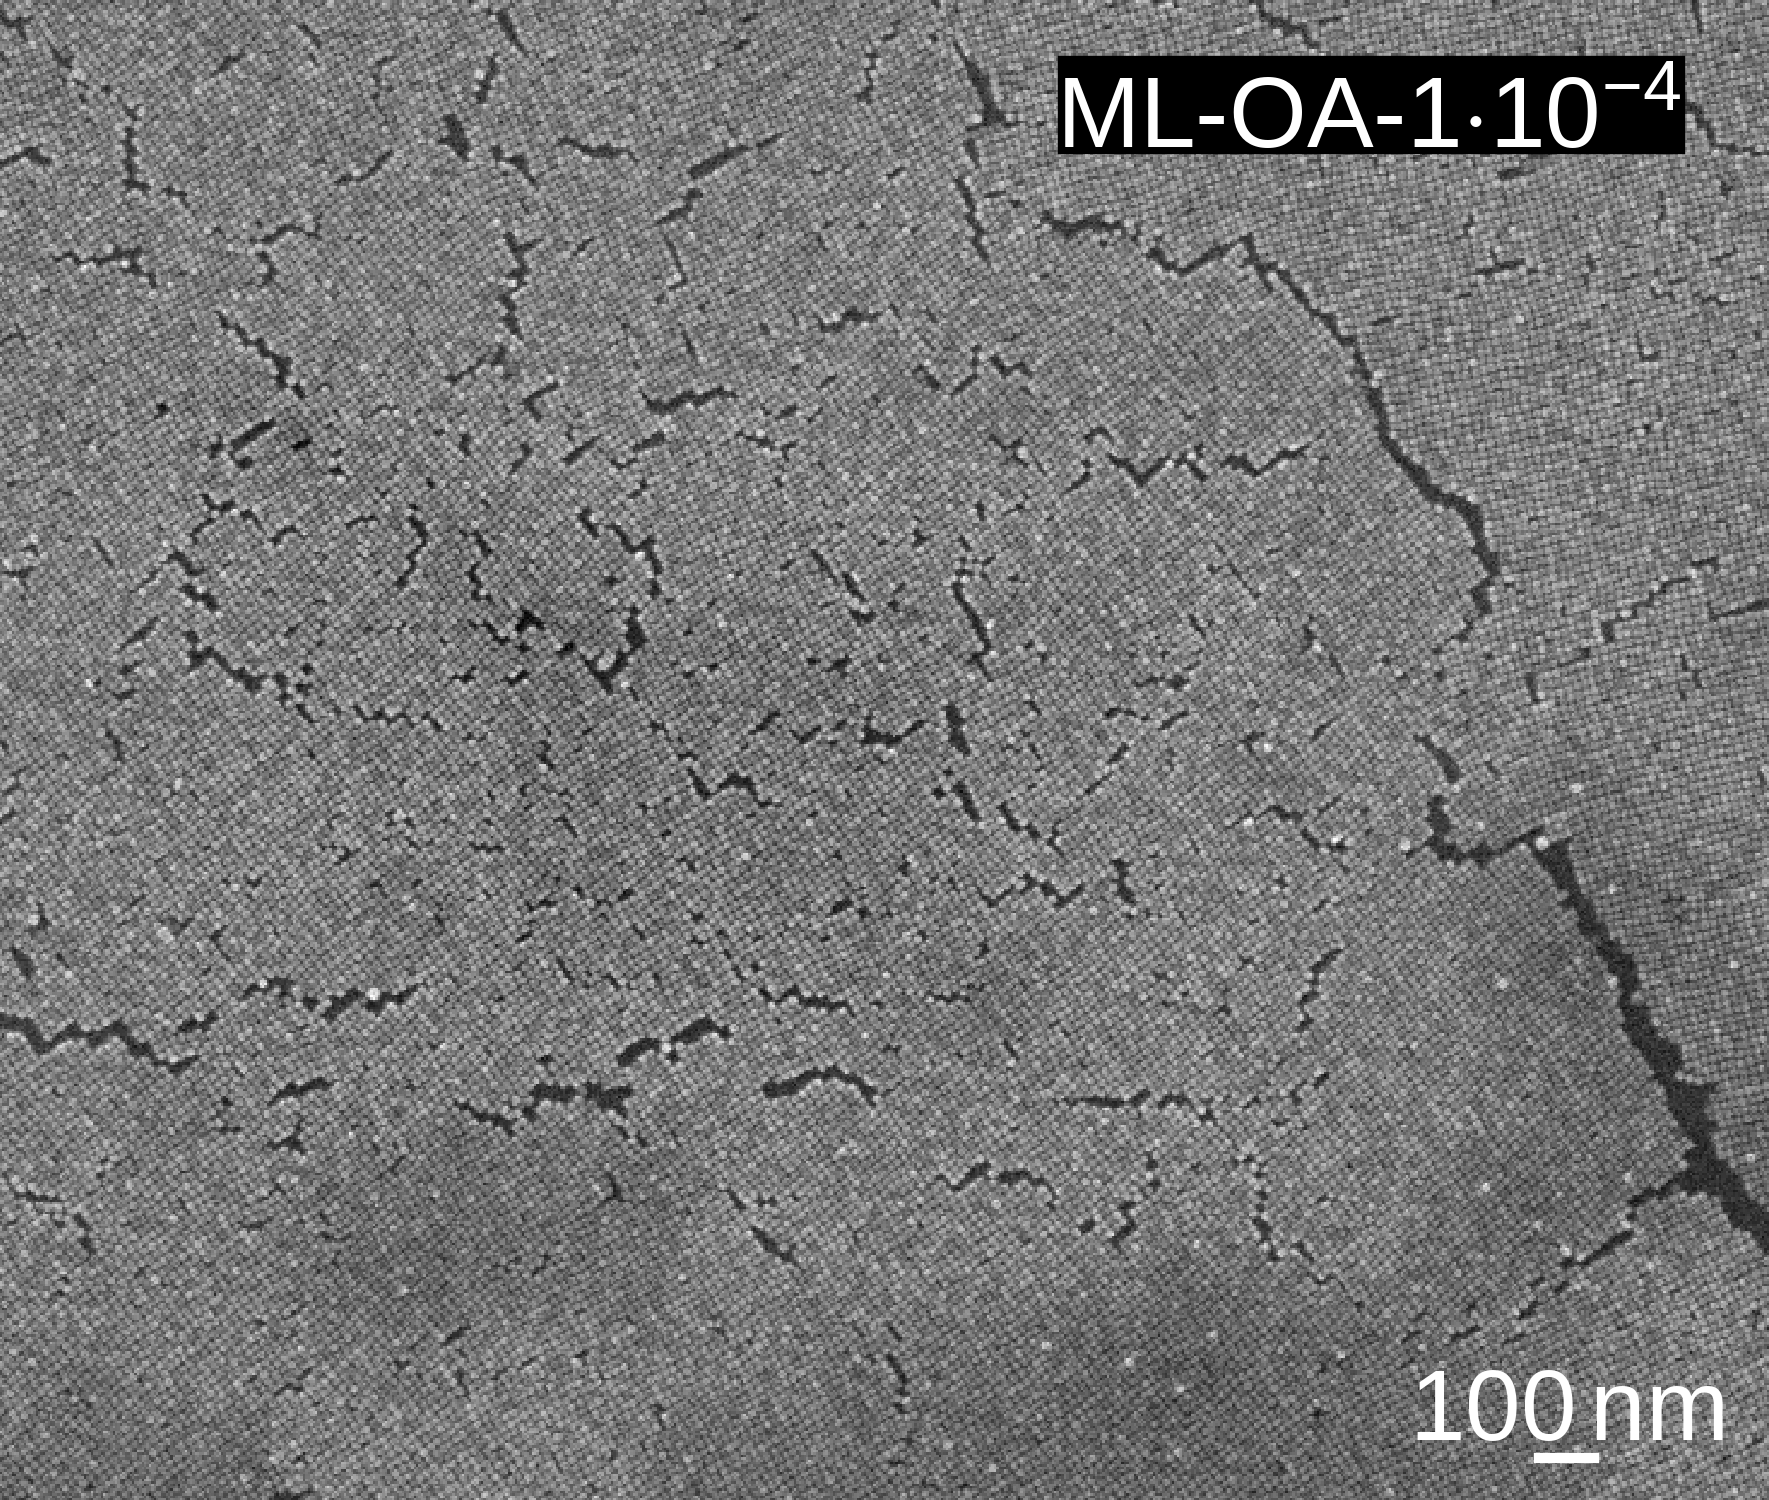
\includegraphics{monolayers_SEM_ML-OA-1e-4}
      \caption{\label{fig:monolayers:preparation:solventVariation:OAAddend}Variation of the oleic acid content analyzed in scanning electron microscopy. Monolayers drop casted from a dispersion of cobalt ferrite nanocubes with $5\cdot10^{-4} \unit{\%}$ (upper left), $1\cdot10^{-3} \unit{\%}$ (upper right), $5\cdot10^{-3} \unit{\%}$ (lower left) and $1\cdot10^{-2} \unit{\%}$ (lower right) oleic acid addend in the dispersion are shown.}
    \end{figure}

    To verify this assumption, a \textit{n}-heptane/1-octadecene dispersion of cobalt ferrite nanocubes, prepared following the the acetylacetonate route, is prepared with a particle concentration of $c_m \eq 0.12 \unit{mg/mL}$ and a 1-octadecene content of $2\unit{\%}$.
    Then, varied amounts of oleic acid are added to the particle dispersion and $V_\textsf{disp} \eq 50 \unit{\unitmu L}$ are drop casted on a clean silicon wafer of $ A_\textsf{wafer} \eq 1 \times 1 \unit{cm^2}$ size.
    The resulting structures are analyzed qualitatively in SEM with exemplarly images shown in \reffig{fig:monolayers:preparation:solventVariation:OAAddend}.
    The images clearly show the trend for increasing long order conditions with increasing the oleic acid content above $c_V^\textsf{OA} \eq 5\cdot10^{-3} \unit{\%}$.
    To put this amount into context, one can estimate which height the oleic acid film would have if it is evenly distributed on the silicon wafer surface by
    \begin{align}
      h \eq \frac{c_V^\textsf{OA} V_\textsf{disp}}{A_\textsf{wafer}}, \label{eq:monolayers:preparation:solventVariation:OAAddend}
    \end{align}
    to $h \eq 25 \unit{nm}$.
    Thus, the needed amount of oleic acid addend within the dispersion to obtain a monolayer formation has as order of magnitude about 2-3 times the nanoparticle size.
    One is limited in the amount that one adds to the dispersion as oleic acid is very difficult to remove from the wafer after the drying of the primary solvent and the 1-octadecene and therefore should be kept minimal.
    It is reasonable to assume that the additional oleic acid during the final drying stage functions as a thin mobilization layer on which the nanocubes can still move in two dimensions, rearrange and reduce the defects in the lattice.

    In summary, the presented data show that a combination of \textit{n}-heptane, 1-octadecene and oleic acid, with fine-tuned ratios, lead to long-range order for oleic acid capped nanoparticles into two dimensional structures that depend on the particle shape.
    It is however important that more parameters are considered during and after the two drying stages to obtain clean and homogeneous monolayers, as is discussed in the following.
\end{document}